\documentclass[a4paper]{cas-sc}

\usepackage[authoryear]{natbib}
\usepackage{setspace}
% Author macros
\def\tsc#1{\csdef{#1}{\textsc{\lowercase{#1}}\xspace}}
\tsc{WGM}
\tsc{QE}

\usepackage{amssymb}
\usepackage{amsmath,amsfonts}
\usepackage{caption}
\captionsetup[figure]{
  name={Fig.},
  labelsep=colon,
  font={rm,small},
  labelfont=bf,
  justification=raggedright,
  singlelinecheck=off,
  skip=4pt,
}
\setlength{\textfloatsep}{8pt plus 2pt minus 2pt}
\setlength{\floatsep}{8pt plus 2pt minus 2pt}
\setlength{\intextsep}{8pt plus 2pt minus 2pt}
\renewcommand{\topfraction}{0.95}
\renewcommand{\bottomfraction}{0.95}
\renewcommand{\textfraction}{0.05}
\renewcommand{\floatpagefraction}{0.8}
% Patch cas-common.sty: replace \sffamily with \rmfamily in caption functions to match body text
\ExplSyntaxOn
\cs_set:Npn \__make_tbl_caption:nn #1#2
{
  \l_tbl_align_tl
  \skip_vertical:N \l_tbl_abovecap_skip
  {\parbox{\dimexpr(\l_tbl_width_dim)}
    {\setstretch{1}\rightskip=0pt\rmfamily\small\textbf{\color{scolor}#1}\par#2\par\vskip2pt}}
  \skip_vertical:N \l_tbl_belowcap_skip
}
\cs_set:Npn \__make_fig_caption:nn #1#2
{
  \l_fig_align_tl
  \skip_vertical:N \l_fig_abovecap_skip
  \setbox\cascaptionbox=\hbox{%
    \setstretch{1}\rmfamily\small\textbf{\color{scolor}#1:}~#2}
  \ifdim\the\wd\cascaptionbox<\dim_use:N \l_fig_width_dim\relax
    \parbox{\l_fig_width_dim}
      {\setstretch{1}\raggedright\unskip\ignorespaces\rmfamily\small\textbf{\color{scolor}#1:}~#2\par}
  \else
    \parbox{\l_fig_width_dim}
      {\setstretch{1}\raggedright\unskip\ignorespaces\rmfamily\small\textbf{\color{scolor}#1:}~#2\par}
  \fi
  \skip_vertical:N \l_fig_belowcap_skip
}
% Patch cas-common.sty: suppress ORCID line and customize first-page footer text
\RenewDocumentCommand \printorcid { } { }
\cs_set:Npn \__first_footerline:
{
  \group_begin:
  \scriptsize
  \sffamily
  \ifnum\theblind>0\relax
  \else
    \__short_authors: :~
  \fi
  { \rmfamily \itshape Preprint~submitted~to~Energy }
  \group_end:
}
\ExplSyntaxOff
\usepackage[linesnumbered,ruled]{algorithm2e}
\usepackage{array}
\usepackage{textcomp}
\usepackage{stfloats}
\usepackage{float}
\usepackage{placeins}
\usepackage{url}
\usepackage{verbatim}
\usepackage{graphicx}
\usepackage{epstopdf}
\epstopdfsetup{outdir=./build/}
\graphicspath{{./}{./build/}}
\usepackage{multirow}
\usepackage{mathrsfs}
%\usepackage{mathptmx}
\usepackage{amsthm}
\newtheorem{myDef}{Definition}
\newtheorem{myTheo}{Theorem}
\newtheorem{mypro}{Proposition}
\newtheorem{myex}{Example}
\usepackage{booktabs}
\usepackage{threeparttable}
\usepackage{etoolbox}
\captionsetup[table]{
  labelsep=newline,
  singlelinecheck=false,
  skip=4pt,
}
\AtBeginEnvironment{table}{\rmfamily\normalsize}
\AtBeginEnvironment{table*}{\rmfamily\normalsize}
\AtBeginEnvironment{tabular}{\rmfamily\normalsize}
\usepackage{hyperref}
\hypersetup{%hypertex=true,
            colorlinks=true,
            linkcolor=blue,
            anchorcolor=blue,
            citecolor=blue}
\newtheorem{remark}{Remark}   
\renewcommand{\qedsymbol}{}
\renewcommand{\theenumi}{\arabic{enumi}}
\renewcommand{\labelenumi}{(\theenumi)}
\setlength{\bibsep}{0pt}
\AtBeginEnvironment{thebibliography}{\singlespacing\scriptsize\setlength{\parskip}{0pt}\setlength{\itemsep}{0pt}}

% Keep abstract in main.tex to make SyncTeX jump to the source file.
\makeatletter
\ExplSyntaxOn
\tl_new:N \g__cas_abs_tl

\RenewDocumentEnvironment { abstract } { o +b }
{
  \IfNoValueTF { #1 } { }
   { \tex_gdef:D \abstracttitle { #1 } }
  \tl_gset:Nn \g__cas_abs_tl { #2 }
}
{ }

\AtBeginDocument{\onehalfspacing}

\RenewDocumentCommand \MaketitleBox { O{} }
{
  \tl_if_blank:nTF { #1 } { }
  { \keys_set:nn { stm / mktitle } { #1 } }
  \processbreakafter
  \singlespacing
  \group_begin:
  \@title
  \group_end:
  %
  \bool_if:NTF \g_stm_blind_bool
  { \vspace* { 10 mm } }
  {
    \group_begin:
    \normalsize \stmauthors \par
    \stmcollab \par
    \footnotesize \itshape \stmaddress \par
    \group_end:
    \bool_if:NTF \g_stm_breakafter_auaff_bool
    { \newpage } { }
  }
  % \printFirstPageNotes
  %
  \dashrule{0pt}{3pt}
  \begin{Abstract}
    \noindent \ignorespaces
    \tl_use:N \g__cas_abs_tl
  \end{Abstract}
  \dashrule{6pt}{3pt}
  \bool_if:NTF \g_stm_breakafter_abstract_bool
  { \newpage } { }
  \onehalfspacing
}

\RenewDocumentCommand \LongMaketitleBox { O{} }
{
  \tl_if_blank:nTF { #1 } { }
  { \keys_set:nn { stm / mktitle } { #1 } }
  \vbox_gset:Nn \g_stm_front_box
  {
    \singlespacing
    \group_begin:
    \@title
    \group_end:
    %
    \bool_if:NTF \g_stm_blind_bool
     { \vspace* { 10 mm } }
     { \group_begin:
       \normalsize \stmauthors \par
       \stmcollab \par
       \footnotesize \itshape \stmaddress \par
       \group_end:
     }
  %
  \dashrule{0pt}{3pt}
  \begin{Abstract}
    \noindent \ignorespaces
    \tl_use:N \g__cas_abs_tl
  \end{Abstract}
  \dashrule{3pt}{3pt}
  }
  \vbox_gset:Nn \g_stm_notes_box
  {  \cs_set_eq:NN \footnotetext \__fn_text:n  \printFirstPageNotes }
   \dim_gset:Nn \g_tmpb_dim { \box_ht:N \g_stm_notes_box }
   % \iow_term:x { ...~[ht: \dim_use:N \g_tmpb_dim  ] }
   \dim_gadd:Nn \g_tmpb_dim { \box_dp:N \g_stm_notes_box }
   % \iow_term:x { ...~[ht+dp: \dim_use:N \g_tmpb_dim  ] }
   \ifbool{sc}{\dim_gadd:Nn \g_tmpb_dim { 12pt } } { }
}
\ExplSyntaxOff
\makeatother


\begin{document}
\let\WriteBookmarks\relax
\def\floatpagepagefraction{1}
\def\textpagefraction{.001}

%------------------------ Title ------------------------

% \title [mode = title]{Subspace Learning Based on Cross-Domain Large Margin Distribution Machine}
\title [mode = title]{Transfer Learning Quantile Large-margin Distribution Machine for Wind Power Forecasting under Extreme Events}
\shorttitle{}

%------------------------ Authors ------------------------
% short author
\shortauthors{Junlin Chen et~al.}

%% ---- First Author ----
\author[1]{Junlin Chen}
\credit{Methodology, Software, Writing - original draft}
\affiliation[1]{
    organization={School of Management and Engineering, Nanjing University},
    city={Nanjing},
    citysep={},
    postcode={210093}, 
    country={China}}

\affiliation[2]{
    organization={Department of Information Engineering and Computer Science, Feng Chia University},
    city={Taiwan},
    citysep={},
    postcode={40724}, 
    country={China}}

\affiliation[3]{
    organization={College of Artificial Intelligence, Southwest University},
    city={Chongqing},
    citysep={},
    postcode={400715}, 
    country={China}}

\affiliation[4]{
    organization={Graduate School of Information, Production and Systems, Waseda University},
    city={Kitakyushu},
    citysep={},
    postcode={808-0135}, 
    country={Japan}}

%% ---- Second Author ----
\author[1]{Bo Wang}
\cormark[1]
\credit{Writing -- review $\&$ editing, Funding acquisition}
\cortext[cor1]{Corresponding author: Bo Wang\\
\qquad \qquad E-mail address: jlchen08@163.com (J. Chen), bowangsme@nju.edu.cn (B. Wang), zhihangyu@smail.nju.edu.cn (Z. Yu),\\
\qquad \qquad  linrenju7@163.com (R. Lin), peiclin@fcu.edu.tw (P. Lin), lbzhang@swu.edu.cn (L. Zhang), junzo.watada.ips@gmail.com (J. Watada)
}

%% ---- Third Author ----
\author[1]{Zhihang Yu}
\credit{Formal analysis, Software}

\author[1]{Renju Lin}
\credit{Software}

%% ---- Fourth Author ----
\author[2]{Pei-chun Lin}
\credit{Validation, Supervision}


%% ---- Fifth Author ----
\author[3]{Libo Zhang}
\credit{Funding acquisition}


%% ---- sixth Author ----
\author[4]{Junzo Watada}
\credit{Validation, Supervision}


%------------------------ Abstract ------------------------
\begin{abstract}
Accurate wind power forecasting under extreme events is critical for grid stability and renewable energy integration, yet remains a formidable challenge due to severe data scarcity and substantial distribution shifts between normal and extreme-event operating regimes. While kernel-based methods, particularly support vector regression and Large-margin Distribution Machine-based Regression (LDMR), have demonstrated strong performance in various regression tasks due to their theoretical guarantees and robustness on limited data, their application to extreme-event forecasting faces critical limitations: the i.i.d. assumption underlying standard kernel methods is fundamentally violated under cross-domain scenarios, and the symmetric variance minimization in LDMR implicitly encourages symmetric error distributions, which conflicts with the asymmetric nature of quantile-based interval prediction required for uncertainty quantification. To extend kernel-based regression to extreme-event forecasting, we propose Transfer Learning Quantile Large-margin Distribution Machine for Regression (TL-QLDMR), which addresses these challenges through three synergistic innovations: (i) an asymmetric variance regularizer that preserves LDMR's distributional robustness while accommodating quantile-specific error asymmetry, (ii) a supervised transfer learning framework integrating maximum mean discrepancy for feature alignment and weighted pinball loss for label adaptation, enabling effective knowledge transfer from abundant normal-domain data to scarce extreme-event samples, and (iii) a scalable Nystr\"{o}m-SGD solver reducing complexity from $O(N^3)$ to $O(T \cdot N \cdot m)$. Comprehensive experiments on six wind farms demonstrate that TL-QLDMR achieves competitive performance in both deterministic and probabilistic forecasting in the extreme-event domain, with superior reliability-sharpness trade-off and practical scalability, making it suitable for real-time applications where interpretability and theoretical guarantees are prioritized.
\end{abstract}


%------------------------ Keywords ------------------------
\begin{keywords}
Wind power forecasting\\
Large-margin distribution machine\\
Quantile regression\\
Transfer learning\\
Extreme events
\end{keywords}

\maketitle
%% \linenumbers

%% main text
%------------------------ Introduction ------------------------
\section{Introduction}

The global transition toward renewable energy has positioned wind power as a cornerstone of sustainable electricity generation. However, the inherent intermittency and volatility of wind resources pose significant challenges to power-system reliability, reserve allocation, and dispatch efficiency \citep{yuan2023conditional}. Accurate wind power forecasting is therefore critical for reducing balancing costs, supporting storage planning, and enabling secure grid integration \citep{yan2025economic, wang2025ensemble}. While substantial progress has been achieved in short-term forecasting under normal meteorological conditions, prediction performance can degrade significantly during extreme events, particularly those associated with typhoons, cold waves, or heat waves, when wind power fluctuations are most severe and energy-system operations are under the greatest stress \citep{wang2024scarcity, jonkers2024regional}.

Extreme events present a dual challenge for data-driven forecasting models. First, such events are inherently rare, resulting in severe data scarcity: extreme-condition samples typically constitute only a small fraction of historical records \citep{s41597-022-01696-6, wang2024scarcity}. Second, the dynamics under extreme-event conditions differ fundamentally from normal operating regimes, inducing substantial distribution shifts in both feature space (e.g., wind speed, temperature) and label space. In this work, the term extreme events is used in a broad operational sense: it includes, but is not limited to, named severe-weather processes and instead denotes rare, high-risk, and out-of-distribution states induced by extreme meteorological deviations and their associated turbine responses. For instance, during typhoon events, wind speeds may exceed 25 m/s, triggering turbine cut-out operations that produce near-zero power output---a pattern rarely observed in normal-domain training data. This creates a covariate shift in the input space and a label shift in the output space, both of which challenge conventional machine learning models that assume training and testing data are independently and identically distributed (i.i.d.) \citep{dong2023mdan, yin2021serioparallel}.

Among the diverse landscape of forecasting methodologies, kernel-based approaches—particularly Support Vector Regression (SVR) and its variants—have been extensively applied to wind power forecasting and have demonstrated competitive performance under normal-operating conditions \citep{wang2019review, li2021cuckoo, luo2024fsvr, yuan2022jellyfish}. The SVR methodology continues to evolve, with recent advances in optimization algorithms, convergence properties, and robustness enhancements. These kernel methods offer several distinctive advantages over black-box deep learning models: strong generalization guarantees rooted in statistical learning theory, effective handling of high-dimensional feature spaces through the kernel trick, convex optimization formulations that guarantee global optima, and robust performance on small-to-medium-sized datasets where deep models tend to overfit. Moreover, their interpretability and theoretical foundations make them particularly attractive for safety-critical applications such as grid dispatch, where model transparency is often required by regulatory standards. Recent studies have further enriched kernel regression through robust SVM formulations \citep{trafalis2006robust}, bounded-loss regression \citep{fu2023bounded}, and multiple-kernel learning with compound regularization \citep{jiang2021rlmkl}, reinforcing the continuing relevance of robustness-oriented kernel learning for forecast tasks involving noisy and heterogeneous data.

Despite these strengths, existing kernel-based wind power forecasting studies predominantly focus on normal-operating conditions with deterministic point prediction objectives. Traditional SVR minimizes the $\epsilon$-insensitive loss to estimate the conditional mean, achieving robust point predictions under Gaussian noise assumptions. More generally, direct quantile-based forecasting has long been recognized as an effective route to interval generation under skewed and heteroscedastic demand patterns \citep{taylor2007ewqr}. To address the need for uncertainty quantification, Support Vector Quantile Regression (SVQR) extends SVR by replacing the symmetric $\epsilon$-loss with the asymmetric pinball loss, enabling estimation of conditional quantiles for prediction intervals \citep{ye2025nfs, tsvqr2023}. Recent SVQR variants incorporate twin-hyperplane designs \citep{tsvqr2023}, robustness-enhancing loss formulations \citep{wang2024ssvqr}, and nonlinear feature selection \citep{ye2025nfs} to improve scalability and robustness. Despite these methodological advances, the application of kernel-based methods to extreme-event forecasting remains largely unexplored, presenting both challenges and opportunities for methodological extension.

At the methodological level, a fundamental limitation shared by both SVR and SVQR is that they optimize only the minimum margin while ignoring the statistical distribution of margins across the entire dataset. This focus on worst-case samples can lead to overfitting and poor generalization, particularly when training data contains outliers or label noise. To overcome this limitation, the Large-margin Distribution Machine-based Regression (LDMR) paradigm was introduced, which explicitly optimizes both the mean and variance of the margin distribution \citep{zhang2019optimal, gupta2021least}. By concentrating prediction errors tightly around zero, LDMR achieves superior generalization compared to classical SVR on a wide range of regression tasks \citep{gupta2021least, hazarika2023mode}. Variants of LDMR have been successfully applied to wind turbine fault detection \citep{tang2019cost}, imbalanced classification \citep{CHENG2016107}, and structural health monitoring \citep{doi:10.1177/14759217231159948}, demonstrating its robustness in noisy industrial environments. However, LDMR has not been systematically applied to wind power forecasting, particularly under extreme-event conditions where both distributional robustness and probabilistic interval prediction are required. These characteristics---combined with LDMR's theoretical foundations---make it a promising candidate for extension to forecasting in the extreme-event domain.

Against this backdrop, extending kernel-based methods from the normal-operating domain to the extreme-event domain introduces three critical challenges that require methodological innovation. First, the i.i.d. assumption---that training and testing data are drawn from the same distribution---is a foundational premise of both SVR/SVQR and LDMR. While this assumption holds reasonably well within a single operating regime, it is systematically violated when transferring knowledge from normal (source domain) to extreme-event (target domain) conditions. For example, in our preliminary analysis of six wind farms, the Wasserstein distance between normal and extreme power distributions ranges from 5.96 to 21.06, indicating substantial distributional discrepancy. A model trained solely on abundant normal-domain data will inevitably exhibit performance degradation when deployed under extreme conditions, regardless of how well the margin distribution is optimized within the source domain. Recent wind-power studies have explored transfer learning and domain adaptation to alleviate data scarcity and domain shift in newly built or heterogeneous wind farms \citep{yin2021serioparallel, wang2024scarcity, dong2023mdan}; however, their principled integration with kernel-based regression remains an open research question.

Second, there exists a fundamental theoretical tension between LDMR's distributional robustness mechanism and the requirements of quantile regression. The core principle of LDMR—minimizing the variance of prediction residuals—implicitly encourages a symmetric, concentrated error distribution around zero. This is theoretically appropriate and empirically effective for conditional mean estimation, as evidenced by LDMR's superior performance over SVR in numerous regression benchmarks. However, quantile regression at level $\tau \neq 0.5$ requires an inherently asymmetric residual distribution: for example, when estimating the 95th percentile, approximately 95\% of errors should be negative and only 5\% positive. Naively applying LDMR's variance minimization to quantile regression will force the error distribution toward symmetry, thereby degrading interval calibration and violating the target coverage probability. This theoretical conflict has received limited attention in the literature, as existing LDMR studies focus primarily on mean regression, and existing SVQR studies do not incorporate distributional robustness. Reconciling these two objectives—distributional robustness and quantile-specific asymmetry—requires a principled modification of the LDMR framework.

Third, existing transfer learning approaches for wind power forecasting predominantly adopt unsupervised or weakly supervised adaptation strategies, focusing primarily on aligning feature distributions while underutilizing scarce target-domain labels \citep{yin2021serioparallel, wang2024scarcity, dong2023mdan}. This design choice is reasonable when target labels are completely unavailable, but is suboptimal for extreme-event forecasting, where scarce target samples represent high-value information that captures critical domain-specific dynamics such as cut-out behavior and power curtailment. A more effective transfer learning framework should leverage both feature-space alignment and label-space supervision, strategically weighting target samples to guide model adaptation. This supervised transfer learning paradigm has been successfully applied in computer vision and natural language processing, but its integration with kernel-based quantile regression for wind power forecasting remains unexplored.

To address these challenges and extend kernel-based regression to extreme-event forecasting, Transfer Learning Quantile Large-margin Distribution Machine for Regression (TL-QLDMR) is proposed as a principled extension of the classical LDMR paradigm for cross-domain probabilistic wind power prediction. The resulting framework preserves the theoretical strengths of kernel-based methods---convex optimization, generalization guarantees, and robustness on limited data---while introducing three synergistic innovations tailored to the extreme-event setting.

First, a novel asymmetric variance regularization mechanism is introduced to reconcile the tension between distributional robustness and quantile estimation. Unlike standard LDMR, which implicitly encourages symmetric error distributions through variance minimization, the proposed formulation employs asymmetric variance regularization based on algebraic residuals, thereby compressing overall error dispersion while preserving the requisite skewness for accurate quantile prediction. This innovation enables TL-QLDMR to achieve both superior point prediction accuracy and well-calibrated prediction intervals, a capability that neither standard LDMR nor SVQR alone can provide.

Second, a supervised transfer learning framework is developed to integrate two complementary adaptation mechanisms. In the feature space, Maximum Mean Discrepancy (MMD) minimization aligns the source and target distributions in the Reproducing Kernel Hilbert Space (RKHS), reducing covariate shift and ensuring that the learned feature representation is domain-invariant \citep{TAO20123962}. In the label space, a weighted pinball loss mechanism assigns substantially higher weights to scarce target-domain samples, treating them as high-value corrective anchors that guide the model toward extreme-event dynamics. This dual-space adaptation strategy enables TL-QLDMR to leverage abundant source data for structural learning while prioritizing target data for domain-specific refinement, thereby addressing the label-neglect problem in existing unsupervised domain adaptation methods. This is particularly important for extreme-event forecasting, where every extreme sample carries valuable information about rare but critical operating conditions such as cut-out events and power curtailment.

Third, because the standard quadratic programming (QP) formulation of kernel-based transfer learning incurs $O(N^3)$ computational complexity through full kernel-matrix computation and inversion, a scalable Nystr\"{o}m-SGD algorithm is developed by combining Nystr\"{o}m approximation---which constructs an explicit low-rank feature mapping using $m \ll N$ landmark points---with stochastic gradient descent (SGD). The resulting complexity is reduced to $O(T \cdot N \cdot m)$, enabling practical deployment on large-scale supervisory control and data acquisition (SCADA) datasets \citep{s41597-022-01696-6} that accumulate tens of thousands of samples annually.

TL-QLDMR is evaluated on a publicly available multi-site wind farm SCADA dataset encompassing six wind farms with capacities ranging from 36 MW to 200 MW, in comparison with recent kernel-based methods, ensemble approaches, and deep learning baselines. Experimental results demonstrate that TL-QLDMR achieves competitive performance in both deterministic and probabilistic forecasting in the extreme-event domain, with consistent improvements across multiple evaluation metrics. Ablation studies confirm the contribution of each component, and scalability analysis validates the efficiency of the proposed Nystr\"{o}m-SGD solver.

% It is important to clarify the scope and positioning of this work. TL-QLDMR is designed for scenarios where kernel-based methods' distinctive advantages---theoretical guarantees, interpretability, sample efficiency, and convex optimization---are particularly valuable. Such scenarios are common in practice: (i) extreme events are inherently rare, providing limited training data where kernel methods' sample efficiency is advantageous, (ii) grid dispatch applications often require model transparency for regulatory compliance, and (iii) real-time forecasting systems benefit from the computational efficiency and stability of convex optimization. Our contribution is to extend the LDMR framework with quantile-aware asymmetry and supervised domain adaptation, demonstrating that kernel-based methods, when properly extended, remain a competitive and theoretically grounded choice for extreme-event forecasting.

The remainder of this paper is organized as follows. Section~\ref{rel} reviews the theoretical foundations of SVQR, LDMR, and transfer learning with MMD, establishing the building blocks for our method. Section~\ref{novel} presents the TL-QLDMR formulation, including the asymmetric variance regularizer, supervised transfer framework, and scalable optimization algorithm. Section~\ref{Experiments} describes the dataset, experimental setup, and comprehensive evaluation results across deterministic prediction, probabilistic interval forecasting, ablation studies, and computational efficiency analysis. Finally, Section~\ref{conclusion} concludes the paper and discusses future research directions.


%------------------------ Related work ------------------------

\section{Related Work}\label{rel}
This section briefly reviews the theoretical foundations related to the proposed method, including Support Vector Quantile Regression, Large-margin Distribution Machine-based Regression, and Transfer Learning with Maximum Mean Discrepancy.

\subsection{Support Vector Quantile Regression}
Traditional SVR relies on the $\epsilon$-insensitive loss function, which assumes a symmetric error distribution (e.g., Gaussian) and estimates the conditional mean of the target variable. However, in scenarios like partial shading or wind curtailment, the noise distribution is often asymmetric and heteroscedastic. To address this, SVQR was introduced to estimate conditional quantiles, providing a comprehensive view of the outcome distribution.
Recent SVQR-family developments include twin-hyperplane designs, robustness-enhancing loss formulations, and nonlinear feature-selection variants, which improve scalability and robustness in non-Gaussian environments \citep{tsvqr2023, wang2024ssvqr, ye2025nfs}.

The core of SVQR is the non-symmetric pinball loss function, defined as
\begin{equation}
L_{\tau}(u) = \begin{cases} 
\tau u, & u \ge 0 \\ 
(\tau - 1) u, & u < 0 ,
\end{cases}
\end{equation}
where $\tau \in (0,1)$ indicates the target quantile. Unlike SVR, SVQR finds a decision boundary that divides the data such that a proportion $\tau$ of the samples lie below the boundary. The optimization problem minimizes the structural risk along with the empirical risk measured by the pinball loss
\begin{equation}
\min_{\boldsymbol{w}, b} \frac{1}{2} \|\boldsymbol{w}\|^2 + C \sum_{i=1}^{n} L_{\tau}(y_i - (\boldsymbol{w}^T \phi(\boldsymbol{x}_i) + b)),
\end{equation}
this formulation allows SVQR to capture heavy-tailed distributions and outliers more effectively than mean-based regression.

\subsection{Large-margin Distribution Machine-based Regression}
While SVR and SVQR focus on maximizing the minimum margin, they largely ignore the statistical distribution of the margin over the entire dataset. LDMR was proposed to improve generalization by explicitly optimizing the distribution of the margins.
From early large-margin distribution formulations to least-squares and mode-seeking variants, LDMR has evolved into a practical framework for robust learning under noisy conditions \citep{zhang2014large, zhang2019optimal, gupta2021least, hazarika2023mode}.

The key idea of LDMR is to not only maximize the margin of the support vectors but also to minimize the variance of the error distribution for all samples. A typical LDMR formulation for regression integrates two additional statistical regularization terms into the objective function
\begin{equation}
\label{eq:ldmr_concept}
\min_{\boldsymbol{w}, b} \frac{1}{2} \|\boldsymbol{w}\|^2 + \lambda_1 \text{Var}(\text{Residuals}) + \lambda_2 \text{Mean}(\text{Residuals}) + C \sum_{i=1}^{n} L(y_i, f(\boldsymbol{x}_i)),
\end{equation}
by constraining the variance, LDMR forces the prediction errors to be clustered tightly around zero, leading to a more compact and robust hypothesis space. However, this variance minimization implicitly encourages symmetric error distributions. Our work extends this concept by introducing an asymmetric variance regularization mechanism suitable for quantile regression, which preserves the distributional robustness of LDMR while accommodating the inherent asymmetry required for accurate quantile estimation.

\subsection{Transfer Learning and Maximum Mean Discrepancy}
Standard machine learning models operate under the assumption that training (source) and testing (target) data are drawn from the same probability distribution. When this assumption is violated---such as in wind power forecasting across different operating regimes---the model performance degrades significantly. Transfer learning aims to transfer knowledge from a label-rich source domain to a target domain with different but related distributions.
MMD-based adaptation has been widely used in transfer scenarios because it provides a non-parametric discrepancy measure in RKHS and integrates naturally with kernelized objectives \citep{TAO20123962, YAN2022107664, GUO2022118237, dp2, ss2}.

A fundamental challenge in transfer learning is measuring and reducing the distribution discrepancy. MMD is a widely used non-parametric metric that measures the distance between two distributions in a RKHS. Given source data $\{\boldsymbol{x}_{S,i}\}$ and target data $\{\boldsymbol{x}_{T,j}\}$, the squared MMD distance is defined as
\begin{equation}
\text{MMD}^2(D_S, D_T) = \left\| \frac{1}{n_S} \sum_{i=1}^{n_S} \phi(\boldsymbol{x}_{S,i}) - \frac{1}{n_T} \sum_{j=1}^{n_T} \phi(\boldsymbol{x}_{T,j}) \right\|_{\mathcal{H}}^2 ,
\end{equation}
where $\phi(\cdot)$ is the feature mapping induced by the kernel. By minimizing the MMD distance during training, the model learns a feature representation where the source and target domains are statistically aligned, enabling the classifier or regressor trained on the source domain to generalize well to the target domain. This alignment is particularly crucial for extreme-event forecasting, as it ensures that the learned predictor is robust to the feature-space shift between normal and extreme-event regimes.


\section{Proposed Method}\label{novel}
This section presents the construction of TL-QLDMR. Necessary notation is introduced first, followed by the final objective function integrating structural risk, distribution variance, domain adaptation, and weighted pinball loss. The constraints required to handle the non-differentiability of the quantile loss are then described.

\subsection{Notations}\label{not}
Consider the problem of wind power forecasting under extreme events. The source domain is denoted by $D_{S} = \{(\boldsymbol{x}_{S,i}, y_{S,i})\}_{i=1}^{n_S}$ and contains abundant normal-operating samples, while the target domain is denoted by $D_{T} = \{(\boldsymbol{x}_{T,j}, y_{T,j})\}_{j=1}^{n_T}$ and contains scarce extreme-event samples. The input space $\mathcal{X} \subseteq \mathbb{R}^d$ represents feature vectors constructed via sliding window processing, and the output space $\mathcal{Y} \subseteq \mathbb{R}$ represents wind power. The sample sizes satisfy $n_T \ll n_S$.

Due to drastic meteorological changes during extreme events, the joint distributions differ significantly: $P_S(\boldsymbol{X}_S, \boldsymbol{Y}_S) \neq P_T(\boldsymbol{X}_T, \boldsymbol{Y}_T)$. This distribution discrepancy implies that a model trained solely on $P_S$ will fail on $P_T$.
A feature mapping $\phi: \mathcal{X} \to \mathcal{H}$ is used to map the input to a high-dimensional Reproducing Kernel Hilbert Space (RKHS). The prediction model is defined as
\begin{equation}
f(\boldsymbol{x}) = \boldsymbol{w}^T \phi(\boldsymbol{x}) + b,
\end{equation}
where $\boldsymbol{w}$ is the weight vector and $b$ is the bias. The quantile $\tau \in (0, 1)$ is set to a specific value (e.g., $\tau=0.95$) for interval prediction (e.g., predicting the upper bound).
Unless otherwise noted, $k(\cdot,\cdot)$ denotes the scalar kernel function, $\boldsymbol{K}$ denotes the Gram matrix, $\phi(\cdot)$ denotes the implicit RKHS mapping used in the exact kernel formulation, and $\psi(\cdot)$ denotes the explicit Nystr\"{o}m feature map used only in the scalable primal solver.

\subsection{TL-QLDMR Model Formulation}\label{MODEL}
The overall architecture of the proposed TL-QLDMR model is illustrated in Fig. \ref{fig:framework}. The left column presents a five-stage pipeline progressing from cross-domain data preparation through supervised transfer, quantile-aware objective construction, scalable optimization, to forecast outputs. In the supervised transfer stage, a shared kernel representation $\phi(\mathbf{x})$/$\psi(\mathbf{x})$ branches into two complementary adaptation paths: feature-space alignment via MMD in RKHS and label-space adaptation via target-weighted pinball loss. The quantile-aware objective integrates four terms---structural risk, asymmetric distribution variance, MMD-based domain adaptation, and weighted pinball loss---into a unified formulation. The optimization stage supports both an exact dual QP solver and a scalable Nystr\"{o}m-SGD solver, ultimately producing point forecasts and probabilistic prediction intervals.

\begin{figure}
\centering
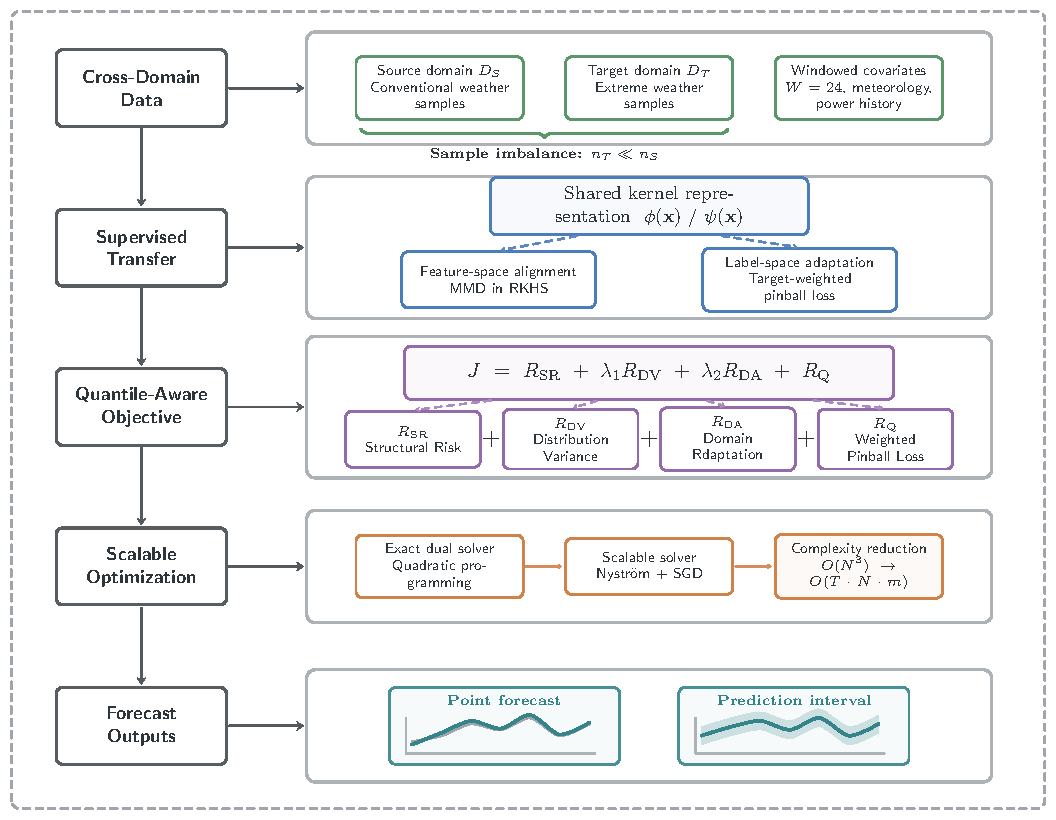
\includegraphics[width=\textwidth]{build/framework.pdf}
\caption{Overall architecture of the proposed TL-QLDMR model. The left column shows the five-stage pipeline: cross-domain data preparation, supervised transfer learning, quantile-aware objective construction, scalable optimization, and forecast outputs. Each stage is elaborated in the corresponding right panel. In the supervised transfer stage, the shared kernel representation branches into feature-space alignment via MMD in RKHS and label-space adaptation via target-weighted pinball loss (indicated by dashed arrows). The quantile-aware objective decomposes into four additive terms: structural risk $R_{\mathrm{SR}}$, distribution variance $R_{\mathrm{DV}}$, domain adaptation $R_{\mathrm{DA}}$, and weighted pinball loss $R_{\mathrm{Q}}$. The optimization stage provides both an exact dual QP solver and a scalable Nystr\"om-SGD solver with complexity reduction from $O(N^3)$ to $O(T \cdot N \cdot m)$. The final outputs include deterministic point forecasts and probabilistic prediction intervals.}
\label{fig:framework}
\end{figure}

\subsubsection{Objective Function}
Our optimization goal is to find the optimal $\boldsymbol{w}, b$ and slack variables $\boldsymbol{\xi}, \boldsymbol{\xi}^*$ to minimize the following objective function $J$. Let $\bar{u}_S = \frac{1}{n_S}\sum_{i=1}^{n_S}(y_{S,i} - f(\boldsymbol{x}_{S,i}))$ denote the mean residual over the source domain, which is treated as a scalar constant during optimization
\begin{equation}
\label{eq:objective}
\begin{aligned}
\min_{\boldsymbol{w}, b, \boldsymbol{\xi}, \boldsymbol{\xi}^*} \quad J = & \underbrace{\frac{1}{2} \|\boldsymbol{w}\|^2}_{\text{(1) Structural Risk}} \\
& + \underbrace{\lambda_1 \sum_{i=1}^{n_S} \left( (y_{S,i} - \boldsymbol{w}^T\phi(\boldsymbol{x}_{S,i}) - b) - \bar{u}_S \right)^2}_{\text{(2) Distribution Variance}} \\
& + \underbrace{\lambda_2 \left\| \frac{1}{n_S} \sum_{i=1}^{n_S} \phi(\boldsymbol{x}_{S,i}) - \frac{1}{n_T} \sum_{j=1}^{n_T} \phi(\boldsymbol{x}_{T,j}) \right\|_{\mathcal{H}}^2}_{\text{(3) Domain Adaptation}} \\
& + \underbrace{C_S \sum_{i=1}^{n_S} L_{\tau}(y_{S,i}, f(\boldsymbol{x}_{S,i})) + C_T \sum_{j=1}^{n_T} L_{\tau}(y_{T,j}, f(\boldsymbol{x}_{T,j}))}_{\text{(4) Weighted Pinball Loss}},
\end{aligned}
\end{equation}
the physical meaning of each term is as follows:
\begin{enumerate}
    \item \textbf{Structural Risk}: This term controls the complexity of the model and prevents overfitting, embodying the maximum margin principle of SVM.
    \item \textbf{Distribution Variance}: This term is the core of our proposed Quantile LDMR model, incorporating a critical modification to the original LDMR variance.
    \begin{itemize}
        \item \textbf{Theoretical Conflict}: The original LDMR minimizes the variance of residuals, which implicitly encourages a symmetric, concentrated error distribution around zero. However, quantile regression at level $\tau \neq 0.5$ requires an asymmetric residual distribution where approximately $\tau$ proportion of errors are negative. Applying a symmetric variance penalty would force the residual distribution towards symmetry, degrading the skewness required for accurate quantile estimation.
        \item \textbf{Asymmetric Modification}: To resolve this, we employ an asymmetric variance regularization based on the algebraic residuals. This design allows the model to reduce error dispersion without constraining the distribution's direction, thereby preserving the non-symmetric properties essential for the Pinball Loss and improving interval coverage.
    \end{itemize}
    \item \textbf{Domain Adaptation (MMD)}: This term aligns source and target feature distributions in RKHS by minimizing mean-embedding discrepancy. This alignment ensures that the learned predictor is robust to the feature-space shift between normal and extreme-event regimes. MMD is chosen because it is non-parametric, computationally tractable, and directly compatible with kernelized optimization.
    \item \textbf{Weighted Pinball Loss}: This term performs label-space adaptation under sample imbalance. Unlike purely unsupervised alignment, the objective explicitly includes target-domain labels:
    \begin{itemize}
        \item \textbf{Label-supervised correction}: extreme-event target labels constrain the model in regions where source-domain trends are no longer reliable (e.g., high wind speed under cut-out operation).
        \item \textbf{Imbalance-aware weighting}: by setting $C_T \gg C_S$, prediction errors on scarce target samples receive stronger penalties, preventing optimization from being dominated by abundant source samples.
    \end{itemize}
\end{enumerate}

\subsubsection{Constraints}
To handle the non-differentiability of the pinball loss, we introduce slack variables $\xi_k, \xi_k^*$ to transform it into linear constraints. These constraints apply uniformly to all samples $k$ in the combined training set $D = D_S \cup D_T$, while domain-specific weighting is handled through $C_S$ and $C_T$ in the objective function
\begin{equation}
\label{eq:constraints}
\begin{cases}
y_k - (\boldsymbol{w}^T\phi(\boldsymbol{x}_k) + b) \le \xi_k, & \forall k \in \{1, \dots, n_S + n_T\} \\
(\boldsymbol{w}^T\phi(\boldsymbol{x}_k) + b) - y_k \le \xi_k^*, & \forall k \in \{1, \dots, n_S + n_T\} \\
\xi_k \ge 0, \quad \xi_k^* \ge 0
\end{cases},
\end{equation}
in the objective function, the term $L_{\tau}(y_k, f(\boldsymbol{x}_k))$ corresponds to $\tau \xi_k + (1-\tau) \xi_k^*$.

\subsection{Model Optimization}\label{optimization}
This section derives the dual problem of TL-QLDMR to enable efficient solution via Quadratic Programming (QP).

\subsubsection{Matrix Reformulation of the Primal Problem}
To facilitate the derivation, the variance term and the MMD term in the objective function [Eq. (\ref{eq:objective})] are rewritten using matrix traces or norms. Let $X = [\boldsymbol{X}_S, \boldsymbol{X}_T]$ denote the entire training set with $N = n_S + n_T$ samples.
For consistency with standard derivations, a coefficient of $1/2$ is added to the variance and MMD terms. The primal objective can be reformulated as
\begin{equation}
\label{eq:primal_matrix}
\min_{\boldsymbol{w}, b, \boldsymbol{\xi}, \boldsymbol{\xi}^*} \quad \frac{1}{2} \|\boldsymbol{w}\|^2 + \frac{\lambda_1}{2} \text{Var}_S(\boldsymbol{w}, b) + \frac{\lambda_2}{2} \text{MMD}^2(\boldsymbol{w}) + \sum_{k=1}^N C_k L_\tau(y_k, f(\boldsymbol{x}_k)),
\end{equation}
where $C_k$ takes value $C_S$ if sample $k \in D_S$ and $C_T$ if $k \in D_T$.

Two auxiliary matrices are introduced to express the variance and MMD terms in Eq. (\ref{eq:primal_matrix}) as quadratic forms of the weights:
\begin{enumerate}
    \item \textbf{Variance Matrix} $\mathbf{S}$: To represent the source-domain variance $\sum_{i \in D_S} (y_{S,i} - f(\boldsymbol{x}_{S,i}) - \bar{u}_S)^2$, we define a centering matrix $\boldsymbol{H}_S = \boldsymbol{I}_{n_S} - \frac{1}{n_S} \boldsymbol{1}_{n_S} \boldsymbol{1}_{n_S}^T$. The variance term can be written as $\| \boldsymbol{H}_S (\boldsymbol{y}_S - \boldsymbol{f}_S) \|^2$. To extend this to the full dataset, we define an $N \times N$ matrix $\mathbf{S}$
    \begin{equation}
    \label{eq:matrix_S}
    \mathbf{S} = \begin{bmatrix} \boldsymbol{H}_S & \mathbf{0} \\ \mathbf{0} & \mathbf{0} \end{bmatrix}.
    \end{equation}
    \item \textbf{MMD Matrix} $\mathbf{M}$: The MMD term represents the distance between means. We define the MMD coefficient matrix $\mathbf{M} \in \mathbb{R}^{N \times N}$ as
    \begin{equation}
    \label{eq:matrix_M}
    M_{ij} = \begin{cases} \frac{1}{n_S^2} & i,j \in D_S \\ \frac{1}{n_T^2} & i,j \in D_T \\ \frac{-1}{n_S n_T} & \text{otherwise} \end{cases}.
    \end{equation}
\end{enumerate}

\subsubsection{Representer Theorem and Kernelization}
According to the representer theorem (\cite{scholkopf2001representer}), the optimal weight vector $\boldsymbol{w}$ lies in the span of the feature mappings of the training samples. Note that the representer theorem applies here because all regularization terms (structural risk, variance, and MMD) can be expressed as functions of inner products in RKHS, preserving the kernel structure. Therefore
\begin{equation}
\label{eq:representer}
\boldsymbol{w} = \sum_{i=1}^{N} \beta_i \phi(\boldsymbol{x}_i) = \boldsymbol{\Phi} \boldsymbol{\beta},
\end{equation}
where $\boldsymbol{\Phi} = [\phi(\boldsymbol{x}_1), \dots, \phi(\boldsymbol{x}_N)]$ is the feature matrix and $\boldsymbol{\beta} = [\beta_1, \dots, \beta_N]^T$ are the coefficients.
Substituting Eq. (\ref{eq:representer}) into the prediction function, we get $f(\boldsymbol{X}) = \boldsymbol{\beta}^T \boldsymbol{K} + b \boldsymbol{1}^T$, where $\boldsymbol{K} = \boldsymbol{\Phi}^T \boldsymbol{\Phi}$ is the $N \times N$ kernel matrix.
Consequently, using Eq. (\ref{eq:matrix_S}) and Eq. (\ref{eq:matrix_M}), the structural risk, variance, and MMD terms can be expressed in terms of $\boldsymbol{\beta}$:
\begin{itemize}
    \item Structural Risk: $\|\boldsymbol{w}\|^2 = \boldsymbol{\beta}^T \boldsymbol{K} \boldsymbol{\beta}$.
    \item Distribution Variance: The quadratic part with respect to $\boldsymbol{\beta}$ is $\boldsymbol{\beta}^T \boldsymbol{K} \mathbf{S} \boldsymbol{K} \boldsymbol{\beta}$. Note that the bias $b$ is eliminated by the centering matrix $\boldsymbol{H}_S$.
    \item Domain Adaptation (MMD): $\text{MMD}^2(\boldsymbol{w}) = \boldsymbol{\beta}^T \boldsymbol{K} \mathbf{M} \boldsymbol{K} \boldsymbol{\beta}$.
\end{itemize}

Combining these, we define the total coefficient matrix $\boldsymbol{\Omega}$
\begin{equation}
\label{eq:Omega}
\boldsymbol{\Omega} = \boldsymbol{K} + \lambda_1 \boldsymbol{K} \mathbf{S} \boldsymbol{K} + \lambda_2 \boldsymbol{K} \mathbf{M} \boldsymbol{K}.
\end{equation}

\begin{remark}
When $\boldsymbol{K}$ is positive definite (which holds for common kernels such as RBF on distinct samples) and $\lambda_1, \lambda_2 > 0$, the matrix $\boldsymbol{\Omega}$ is positive definite. This ensures that $\boldsymbol{\Omega}$ is invertible and the optimization problem is well-posed. The positive definiteness of $\boldsymbol{\Omega}$ also guarantees the strong convexity of the objective function, which is essential for both the dual QP formulation and the convergence analysis of the scalable SGD algorithm.
\end{remark}
By substituting the kernelized terms and Eq. (\ref{eq:Omega}) into Eq. (\ref{eq:primal_matrix}), the kernelized primal problem becomes (ignoring constant terms w.r.t $b$ in variance)
\begin{equation}
\label{eq:kernel_primal}
\min_{\boldsymbol{\beta}, b, \boldsymbol{\xi}, \boldsymbol{\xi}^*} \quad \frac{1}{2} \boldsymbol{\beta}^T \boldsymbol{\Omega} \boldsymbol{\beta} - (\lambda_1 \boldsymbol{K} \mathbf{S} \boldsymbol{Y})^T \boldsymbol{\beta} + \sum_{k=1}^N C_k (\tau \xi_k + (1-\tau)\xi_k^*),
\end{equation}
subject to the constraints from Eq. (\ref{eq:constraints})
\begin{equation}
\label{eq:kernel_constraints}
y_k - (\boldsymbol{K}_k \boldsymbol{\beta} + b) \le \xi_k, \quad (\boldsymbol{K}_k \boldsymbol{\beta} + b) - y_k \le \xi_k^*, \quad \xi_k, \xi_k^* \ge 0.
\end{equation}

\subsubsection{Lagrangian and Dual Problem}
We introduce Lagrange multipliers $\alpha_k, \alpha_k^*, \mu_k, \mu_k^* \ge 0$ for Eq. (\ref{eq:kernel_constraints}). The Lagrangian function $\mathcal{L}$ is constructed as
\begin{equation}
\label{eq:lagrangian}
\begin{aligned}
\mathcal{L} = &\frac{1}{2} \boldsymbol{\beta}^T \boldsymbol{\Omega} \boldsymbol{\beta} - (\lambda_1 \boldsymbol{K} \mathbf{S} \boldsymbol{Y})^T \boldsymbol{\beta} + \sum_{k=1}^N C_k (\tau \xi_k + (1-\tau)\xi_k^*) \\
&- \sum_{k=1}^N \alpha_k (\xi_k - y_k + \boldsymbol{K}_k \boldsymbol{\beta} + b) - \sum_{k=1}^N \alpha_k^* (\xi_k^* + y_k - \boldsymbol{K}_k \boldsymbol{\beta} - b) - \sum (\mu_k \xi_k + \mu_k^* \xi_k^*),
\end{aligned}
\end{equation}
by setting the partial derivatives of Eq. (\ref{eq:lagrangian}) with respect to the primal variables ($b, \boldsymbol{\xi}, \boldsymbol{\xi}^*, \boldsymbol{\beta}$) to zero, along with the complementary slackness and primal feasibility conditions, we obtain the KKT conditions
\begin{align}
    \label{eq:kkt_b} \frac{\partial \mathcal{L}}{\partial b} = 0 & \implies \sum_{k=1}^N (\alpha_k - \alpha_k^*) = 0 \\
    \label{eq:kkt_xi} \frac{\partial \mathcal{L}}{\partial \xi_k} = 0, \frac{\partial \mathcal{L}}{\partial \xi_k^*} = 0 & \implies \alpha_k \in [0, C_k \tau], \quad \alpha_k^* \in [0, C_k (1-\tau)] \\
    \label{eq:kkt_beta} \frac{\partial \mathcal{L}}{\partial \boldsymbol{\beta}} = 0 & \implies \boldsymbol{\Omega} \boldsymbol{\beta} - \lambda_1 \boldsymbol{K} \mathbf{S} \boldsymbol{Y} - \boldsymbol{K} (\boldsymbol{\alpha} - \boldsymbol{\alpha}^*) = 0,
\end{align}
let $\boldsymbol{\gamma} = \boldsymbol{\alpha} - \boldsymbol{\alpha}^*$. From Eq. (\ref{eq:kkt_beta}), the optimal $\boldsymbol{\beta}$ is derived as
\begin{equation}
\label{eq:beta_optimal}
\boldsymbol{\beta} = \boldsymbol{\Omega}^{-1} (\boldsymbol{K} \boldsymbol{\gamma} + \lambda_1 \boldsymbol{K} \mathbf{S} \boldsymbol{Y}).
\end{equation}

Substituting Eq. (\ref{eq:beta_optimal}) back into Eq. (\ref{eq:lagrangian}), and simplifying using Eq. (\ref{eq:kkt_b}) and Eq. (\ref{eq:kkt_xi}), we arrive at the dual Problem, which is a standard Quadratic Programming (QP) problem
\begin{equation}
\label{eq:dual_problem}
\begin{aligned}
\min_{\boldsymbol{\alpha}, \boldsymbol{\alpha}^*} \quad & \frac{1}{2} (\boldsymbol{\alpha} - \boldsymbol{\alpha}^*)^T \mathbf{Q}_{dual} (\boldsymbol{\alpha} - \boldsymbol{\alpha}^*) + \mathbf{p}_{dual}^T (\boldsymbol{\alpha} - \boldsymbol{\alpha}^*) \\
\text{s.t.} \quad & \sum_{k=1}^N (\alpha_k - \alpha_k^*) = 0 \\
& 0 \le \alpha_k \le C_k \tau, \quad \forall k \\
& 0 \le \alpha_k^* \le C_k (1-\tau), \quad \forall k
\end{aligned},
\end{equation}
where the dual matrix $\mathbf{Q}_{dual}$ and vector $\mathbf{p}_{dual}$ are defined as
\begin{equation}
\label{eq:dual_matrices}
\mathbf{Q}_{dual} = \boldsymbol{K} \boldsymbol{\Omega}^{-1} \boldsymbol{K}, \quad \mathbf{p}_{dual} = \lambda_1 \boldsymbol{K} \boldsymbol{\Omega}^{-1} \boldsymbol{K} \mathbf{S} \boldsymbol{Y} - \boldsymbol{Y}.
\end{equation}

Once the optimal $\boldsymbol{\alpha}, \boldsymbol{\alpha}^*$ are found using a QP solver for Eq. (\ref{eq:dual_problem}), we can recover $\boldsymbol{\beta}$ using Eq. (\ref{eq:beta_optimal}) and construct the final decision function $f(\boldsymbol{x})$.


\subsection{The Algorithm and Complexity Analysis}\label{alg_section}
The complete training process of the proposed TL-QLDMR model is summarized in Algorithm \ref{alg:TL-QLDMR}. The algorithm mainly consists of matrix construction and solving a QP problem.

\begin{algorithm}
\SetKwInOut{Input}{Input}
\SetKwInOut{Output}{Output}
\caption{TL-QLDMR Training Algorithm}
\label{alg:TL-QLDMR}
\Input{Source Data $D_S = \{(\boldsymbol{x}_{S,i}, y_{S,i})\}_{i=1}^{n_S}$, Target Data $D_T = \{(\boldsymbol{x}_{T,j}, y_{T,j})\}_{j=1}^{n_T}$, Quantile $\tau$, Kernel parameters, Regularization parameters $\lambda_1, \lambda_2$, Pinball Loss weights $C_S, C_T$.}
\Output{Optimal dual variables $\boldsymbol{\alpha}, \boldsymbol{\alpha}^*$ and bias $b$.}

\tcp{Step 1: Data Preparation}
Combine Source and Target data: $\boldsymbol{X} = [\boldsymbol{X}_S, \boldsymbol{X}_T]$, $\boldsymbol{Y} = [\boldsymbol{Y}_S; \boldsymbol{Y}_T]$, $N = n_S + n_T$\;
Set weights vector $\boldsymbol{C} \in \mathbb{R}^N$ where $C_k = C_S$ for $k \le n_S$ and $C_T$ otherwise\;

\tcp{Step 2: Matrix Construction}
Compute Kernel Matrix $\boldsymbol{K} \in \mathbb{R}^{N \times N}$ using the specified kernel function\;
Construct Variance Matrix $\mathbf{S}$ using Eq. \eqref{eq:matrix_S}\;
Construct MMD Matrix $\mathbf{M}$ using Eq. \eqref{eq:matrix_M}\;

\tcp{Step 3: Dual Problem Formulation}
Compute coefficient matrix $\boldsymbol{\Omega} = \boldsymbol{K} + \lambda_1 \boldsymbol{K} \mathbf{S} \boldsymbol{K} + \lambda_2 \boldsymbol{K} \mathbf{M} \boldsymbol{K}$ using Eq. \eqref{eq:Omega}\;
Invert $\boldsymbol{\Omega}$ to fit the dual form\;
Compute Dual Matrix $\mathbf{Q}_{dual} = \boldsymbol{K} \boldsymbol{\Omega}^{-1} \boldsymbol{K}$ using Eq. \eqref{eq:dual_matrices}\;
Compute Dual Vector $\mathbf{p}_{dual} = \lambda_1 \boldsymbol{K} \boldsymbol{\Omega}^{-1} \boldsymbol{K} \mathbf{S} \boldsymbol{Y} - \boldsymbol{Y}$ using Eq. \eqref{eq:dual_matrices}\;

\tcp{Step 4: Solve QP}
Solve the QP problem in Eq. \eqref{eq:dual_problem} providing $\mathbf{Q}_{dual}$, $\mathbf{p}_{dual}$, and constraints $0 \le \alpha_k \le C_k\tau$, $0 \le \alpha_k^* \le C_k(1-\tau)$\;
\textbf{Return} Optimal $\boldsymbol{\alpha}, \boldsymbol{\alpha}^*$\;

\tcp{Step 5: Recover Primal Variables}
Compute $\boldsymbol{\gamma} = \boldsymbol{\alpha} - \boldsymbol{\alpha}^*$\;
Recover $\boldsymbol{\beta}$ using Eq. \eqref{eq:beta_optimal}\;
Compute bias $b$ using complementary slackness conditions (averaged over Support Vectors)\;
\end{algorithm}

The computational complexity of TL-QLDMR primarily stems from three parts: matrix multiplication, matrix inversion, and the QP solver.
\begin{enumerate}
    \item \textbf{Matrix Operations}: The construction of $\boldsymbol{K}$, $\mathbf{S}$, and $\mathbf{M}$ involves $O(N^2 d)$ or $O(N^2)$ operations. The calculation of $\boldsymbol{\Omega}$ involves matrix multiplications of size $N \times N$, leading to a complexity of $O(N^3)$ in the worst case for dense kernel matrices.
    \item \textbf{Matrix Inversion}: Inverting the $N \times N$ matrix $\boldsymbol{\Omega}$ requires $O(N^3)$ complexity in the worst case.
    \item \textbf{QP Solver}: Solving the standard Quadratic Programming problem for the dual variables typically has a complexity ranging from $O(N^{2.3})$ to $O(N^3)$ depending on the solver implementation (e.g., Interior Point Method).
\end{enumerate}
Therefore, the overall time complexity of the proposed algorithm is approximately $O(N^3)$ in the worst case. Given that $N = n_S + n_T$ and $n_T \ll n_S$, the scale is dominated by the source-domain sample size. While this complexity is acceptable for moderate-sized datasets, it becomes prohibitive for large-scale wind power forecasting scenarios involving tens of thousands of samples. To overcome this computational bottleneck and enable practical deployment in real-world wind farm applications, we develop a scalable optimization algorithm in the following subsection.

\subsection{Scalable Optimization via Nystr\"{o}m Approximation}\label{fast_alg}
To address the computational bottleneck of the standard QP-based solver, we propose a scalable Nystr\"{o}m-SGD algorithm. This approach reduces the time complexity from $O(N^3)$ to $O(T \cdot N \cdot m)$, where $T$ denotes the number of iterations and $m \ll N$ is the number of landmark points.

\subsubsection{Nystr\"{o}m Feature Mapping}
The core idea is to approximate the implicit infinite-dimensional feature mapping $\phi(\boldsymbol{x})$ with an explicit finite-dimensional representation. Given the training data, we first select $m$ landmark points $Z = \{z_1, \ldots, z_m\}$ from the source domain $D_S$ using K-Means clustering to capture the underlying data manifold, following the rationale of clustered Nystr\"{o}m landmark selection \citep{zhang2010clustered}.

Let $\boldsymbol{W} \in \mathbb{R}^{m \times m}$ denote the kernel matrix of landmarks, where $W_{ij} = k(z_i, z_j)$. The explicit feature mapping $\psi: \mathcal{X} \to \mathbb{R}^m$ is then constructed as
\begin{equation}
\label{eq:nystrom_feature}
\psi(\boldsymbol{x}) = \boldsymbol{W}^{-1/2} [k(\boldsymbol{x}, z_1), \ldots, k(\boldsymbol{x}, z_m)]^T,
\end{equation}
where $\boldsymbol{W}^{-1/2}$ is computed via eigendecomposition. This mapping satisfies the approximation property $k(\boldsymbol{x}_i, \boldsymbol{x}_j) \approx \psi(\boldsymbol{x}_i)^T \psi(\boldsymbol{x}_j)$, enabling us to work directly in the primal space.

\subsubsection{Primal Formulation with Explicit Features}
With the explicit feature mapping, the prediction function becomes $f(\boldsymbol{x}) = \boldsymbol{w}^T \psi(\boldsymbol{x}) + b$, where $\boldsymbol{w} \in \mathbb{R}^m$. Let $\boldsymbol{\Psi}_S \in \mathbb{R}^{n_S \times m}$ and $\boldsymbol{\Psi}_T \in \mathbb{R}^{n_T \times m}$ denote the mapped feature matrices for source and target domains, respectively. The regularization matrix $\boldsymbol{R} \in \mathbb{R}^{m \times m}$ incorporating structural risk, variance, and MMD terms is formulated as
\begin{equation}
\label{eq:reg_matrix}
\boldsymbol{R} = \boldsymbol{I} + \lambda_1 \underbrace{\boldsymbol{\Psi}_S^T \boldsymbol{H}_S \boldsymbol{\Psi}_S}_{\text{Variance}} + \lambda_2 \underbrace{(\bar{\boldsymbol{\psi}}_S - \bar{\boldsymbol{\psi}}_T)(\bar{\boldsymbol{\psi}}_S - \bar{\boldsymbol{\psi}}_T)^T}_{\text{MMD}},
\end{equation}
where $\boldsymbol{H}_S = \boldsymbol{I}_{n_S} - \frac{1}{n_S} \boldsymbol{1}_{n_S} \boldsymbol{1}_{n_S}^T$ is the centering matrix, and $\bar{\boldsymbol{\psi}}_S$, $\bar{\boldsymbol{\psi}}_T$ are the mean feature vectors of source and target domains.

\subsubsection{Stochastic Gradient Descent Optimization}
Instead of solving the dual QP problem, we directly optimize the primal objective using the Nystr\"{o}m-SGD procedure. For each sample $k$ in a mini-batch $\mathcal{B}$, the sub-gradient of the Pinball Loss with respect to the prediction is
\begin{equation}
\label{eq:subgradient}
g_k = \frac{\partial L_{\tau}}{\partial \hat{y}_k} = \begin{cases} 
\tau - 1, & \text{if } y_k < \hat{y}_k \\ 
\tau, & \text{if } y_k \ge \hat{y}_k.
\end{cases}
\end{equation}

The weighted sub-gradient is computed as $\tilde{g}_k = C_k \cdot g_k$, where $C_k \in \{C_S, C_T\}$ depends on the domain membership. The parameter gradients are then
\begin{equation}
\label{eq:param_gradients}
\nabla_{\boldsymbol{w}} J = \frac{1}{|\mathcal{B}|} \sum_{k \in \mathcal{B}} \tilde{g}_k \psi(\boldsymbol{x}_k) + \boldsymbol{R} \boldsymbol{w}, \quad \nabla_b J = \frac{1}{|\mathcal{B}|} \sum_{k \in \mathcal{B}} \tilde{g}_k.
\end{equation}

The complete training procedure is summarized in Algorithm \ref{alg:fast_TL-QLDMR}.

\begin{algorithm}[t]
\SetKwInOut{Input}{Input}
\SetKwInOut{Output}{Output}
\caption{TL-QLDMR via Nystr\"{o}m-SGD}
\label{alg:fast_TL-QLDMR}
\Input{Source data $D_S$, Target data $D_T$, Number of landmarks $m$, Quantile $\tau$, Hyperparameters $\lambda_1, \lambda_2, C_S, C_T$, Learning rate $\eta$, Batch size $B$, Max iterations $T$.}
\Output{Optimal weights $\boldsymbol{w} \in \mathbb{R}^m$ and bias $b \in \mathbb{R}$.}

\tcp{Step 1: Nystr\"{o}m Feature Mapping}
Select $m$ landmarks $Z = \{z_1, \ldots, z_m\}$ from $D_S$ via K-Means\;
Compute landmark kernel matrix $\boldsymbol{W} \in \mathbb{R}^{m \times m}$\;
Compute $\boldsymbol{W}^{-1/2}$ via eigendecomposition\;
Construct explicit features $\psi(\boldsymbol{x})$ for all samples using Eq. \eqref{eq:nystrom_feature}\;

\tcp{Step 2: Pre-compute Regularization Matrix}
Compute feature matrices $\boldsymbol{\Psi}_S$, $\boldsymbol{\Psi}_T$ and mean vectors $\bar{\boldsymbol{\psi}}_S$, $\bar{\boldsymbol{\psi}}_T$\;
Construct regularization matrix $\boldsymbol{R}$ using Eq. \eqref{eq:reg_matrix}\;

\tcp{Step 3: Stochastic Optimization}
Initialize $\boldsymbol{w} \leftarrow \boldsymbol{0}$, $b \leftarrow 0$\;
\For{$t = 1$ \KwTo $T$}{
    Shuffle combined dataset $D = D_S \cup D_T$\;
    \For{each mini-batch $\mathcal{B} \subset D$}{
        Compute predictions: $\hat{y}_k = \boldsymbol{w}^T \psi(\boldsymbol{x}_k) + b$, $\forall k \in \mathcal{B}$\;
        Compute sub-gradients $g_k$ using Eq. \eqref{eq:subgradient}\;
        Apply sample weights: $\tilde{g}_k \leftarrow C_k \cdot g_k$\;
        Compute gradients $\nabla_{\boldsymbol{w}} J$, $\nabla_b J$ using Eq. \eqref{eq:param_gradients}\;
        Update $\boldsymbol{w}$, $b$ using the stochastic gradient step with learning rate $\eta$\;
    }
}
\Return $\boldsymbol{w}$, $b$\;
\end{algorithm}

\subsubsection{Complexity Analysis of the Scalable Algorithm}
The proposed scalable algorithm achieves significant computational savings:
\begin{enumerate}
    \item \textbf{Landmark Selection}: K-Means clustering requires $O(N \cdot m \cdot I_{km})$ operations, where $I_{km}$ is the number of K-Means iterations.
    \item \textbf{Feature Mapping}: Computing $\boldsymbol{W}^{-1/2}$ costs $O(m^3)$, and mapping all $N$ samples requires $O(N \cdot m \cdot d)$.
    \item \textbf{Regularization Matrix}: Constructing $\boldsymbol{R}$ involves $O(n_S \cdot m^2)$ for the variance term and $O(m^2)$ for the MMD term.
    \item \textbf{SGD Iterations}: Each iteration processes $O(N)$ samples with $O(m)$ operations per sample, yielding $O(T \cdot N \cdot m)$ total complexity.
\end{enumerate}

The overall time complexity is $O(T \cdot N \cdot m + m^3)$. Since $m \ll N$ (typically $m = O(\sqrt{N})$), this represents a substantial reduction from the $O(N^3)$ complexity of the standard QP solver. Table \ref{tab:complexity} summarizes the comparison between the two algorithms.

\begin{table}[htbp]
\centering
\caption{Complexity comparison between standard QP and scalable algorithm}
\label{tab:complexity}
\begin{tabular}{lcc}
\toprule
\textbf{Component} & \textbf{Standard QP} & \textbf{Scalable (Ours)} \\
\midrule
Kernel/Feature Computation & $O(N^2 d)$ & $O(N m d)$ \\
Matrix Inversion & $O(N^3)$ & $O(m^3)$ \\
Optimization & $O(N^3)$ & $O(T N m)$ \\
\midrule
\textbf{Total} & $O(N^3)$ & $O(T N m + m^3)$ \\
\bottomrule
\end{tabular}
\end{table}

\subsubsection{Theoretical Justification}
The convergence of the proposed Nystr\"{o}m-SGD algorithm is guaranteed under standard assumptions. Since the Pinball Loss is convex and Lipschitz continuous, and the regularization term $\frac{1}{2}\boldsymbol{w}^T \boldsymbol{R} \boldsymbol{w}$ is strongly convex (as $\boldsymbol{R}$ inherits positive definiteness from $\boldsymbol{\Omega}$ when $\lambda_1, \lambda_2 > 0$), the overall objective function is strongly convex. According to the convergence theory of SGD for strongly convex functions \citep{bottou2018optimization}, the algorithm converges to the global optimum at a rate of $O(1/T)$.

Furthermore, the Nystr\"{o}m approximation error is bounded. Let $\tilde{k}(\boldsymbol{x}_i, \boldsymbol{x}_j) = \psi(\boldsymbol{x}_i)^T \psi(\boldsymbol{x}_j)$ denote the approximated kernel. Standard analyses of the Nystr\"{o}m method show that the approximation error decreases with the number of landmarks under suitable spectral assumptions and sampling schemes \citep{kumar2012sampling, zhang2010clustered}. A representative order characterization is
\begin{equation}
\label{eq:nystrom_error}
\mathbb{E}\left[ \| \boldsymbol{K} - \tilde{\boldsymbol{K}} \|_F \right] \le O\left( \frac{N}{\sqrt{m}} \right),
\end{equation}
this bound ensures that with a sufficient number of landmarks, the approximation quality is well-controlled, and the solution obtained by the scalable algorithm closely approximates that of the exact QP solver.


%------------------------- Experiments --------------------%
%------------------------ Experiments Section for TLQLDMR Paper ------------------------%
\section{Experiments}\label{Experiments}

In this section, we conduct a comprehensive experimental evaluation of the proposed TLQLDMR model for wind power forecasting under extreme weather conditions. The experiments are organized into three progressive stages: (1) extreme weather sample screening and domain shift quantification across multiple wind farms (Experiment~1); (2) deterministic point prediction comparison on the wind farm exhibiting the most severe distribution shift (Experiment~2); and (3) probabilistic interval prediction evaluation under a 95\% confidence level (Experiment~3). We first describe the dataset and experimental setup in Sections~\ref{sec:data} and~\ref{sec:setup}, then present the results and analysis in Sections~\ref{sec:exp1}--\ref{sec:exp3}.

%---------------- Dataset Description --------------------%
\subsection{Dataset Description}\label{sec:data}

The experiments are conducted on a publicly available wind farm SCADA dataset published by the State Grid Renewable Energy Generation Dataset \citep{s41597-022-01696-6}. The dataset contains supervisory control and data acquisition (SCADA) records from six onshore wind farms with nominal capacities ranging from 36\,MW to 200\,MW. Each record is sampled at 15-minute intervals and includes the following meteorological and operational variables:

\begin{itemize}
    \item Wind speed at multiple heights: hub height, 50\,m, 30\,m, and 10\,m (m/s);
    \item Wind direction at hub height (degrees);
    \item Air temperature ($^\circ$C);
    \item Atmospheric pressure (hPa);
    \item Relative humidity (\%);
    \item Active power output (MW).
\end{itemize}

Table~\ref{tab:farm_summary} summarizes the basic characteristics of the six wind farms. Each farm contains approximately 70{,}000 time-stamped records spanning multiple years of continuous operation.

\begin{table}[ht]
\centering
\caption{Summary of wind farm sites used in the experiments.}
\setlength{\tabcolsep}{4mm}
\begin{tabular}{cccc}
\toprule
Farm ID & Site Name & Nominal Capacity (MW) & Total Samples \\
\midrule
1 & Wind farm site 1 & 99  & $\sim$70{,}000 \\
2 & Wind farm site 2 & 200 & $\sim$70{,}000 \\
3 & Wind farm site 3 & 99  & $\sim$70{,}000 \\
4 & Wind farm site 4 & 66  & $\sim$70{,}000 \\
5 & Wind farm site 5 & 36  & $\sim$70{,}000 \\
6 & Wind farm site 6 & 96  & $\sim$70{,}000 \\
\bottomrule
\end{tabular}
\label{tab:farm_summary}
\end{table}


%---------------- Feature Engineering --------------------%
\subsection{Feature Engineering and Data Preprocessing}\label{sec:features}

The feature set comprises multi-height wind speeds, air temperature, atmospheric pressure, relative humidity, and cyclically encoded wind direction. Specifically, the raw wind direction angle $\theta$ is transformed into two orthogonal components $\sin(\theta)$ and $\cos(\theta)$ to eliminate the discontinuity at the $0^\circ/360^\circ$ boundary, which is a well-established practice in meteorological feature engineering \citep{wang2019review}.

A sliding window of length $W = 24$ (corresponding to a 6-hour lookback horizon at 15-minute resolution) is applied to construct supervised learning samples. For each window, the feature matrix $\boldsymbol{X}_t \in \mathbb{R}^{W \times d}$ is flattened into a vector $\boldsymbol{x}_t \in \mathbb{R}^{Wd}$, and the target variable $y_t$ is the power output at the next time step. All features and the target variable are standardized to zero mean and unit variance using statistics computed from the training set. Missing values are imputed with the per-feature mean to ensure numerical stability for kernel-based models.

%---------------- Extreme Weather Definition --------------------%
\subsection{Extreme Weather Event Definition}\label{sec:extreme_def}

A critical prerequisite for evaluating transfer learning under extreme conditions is the rigorous definition of what constitutes an ``extreme weather event.'' We adopt a rule-based identification scheme that combines statistical thresholds with physical domain knowledge. A sample is classified as belonging to the \textit{target domain} (extreme weather) if it satisfies any of the following criteria:

\begin{enumerate}
    \item \textbf{Statistical wind speed extreme}: Hub-height wind speed exceeds the 98th percentile of the farm's historical distribution;
    \item \textbf{Temperature extreme}: Air temperature falls below the 2nd percentile or exceeds the 98th percentile;
    \item \textbf{Cut-out wind speed}: Hub-height wind speed exceeds 25\,m/s, the typical cut-out threshold for modern wind turbines.
\end{enumerate}

Notably, the power ramp criterion (rapid power fluctuations exceeding 5\% of nominal capacity per 15-minute interval) is deliberately excluded from the extreme definition. This design choice avoids conflating control-induced power curtailment or dispatch adjustments with genuinely weather-driven anomalies. The union of the above three rules yields a target domain that is both physically interpretable and statistically sufficient for model training. All remaining samples constitute the \textit{source domain} (normal weather conditions).

%---------------- Experimental Setup --------------------%
\subsection{Experimental Setup}\label{sec:setup}

\subsubsection{Evaluation Metrics}

For deterministic point prediction (Experiment~2), we employ the following metrics. Let $y_i$ and $\hat{y}_i$ denote the true and predicted power values, respectively, for $i = 1, \ldots, n$:

\begin{itemize}
    \item \textbf{Root Mean Squared Error (RMSE)}: $\text{RMSE} = \sqrt{\frac{1}{n}\sum_{i=1}^{n}(y_i - \hat{y}_i)^2}$
    \item \textbf{Mean Absolute Error (MAE)}: $\text{MAE} = \frac{1}{n}\sum_{i=1}^{n}|y_i - \hat{y}_i|$
    \item \textbf{Coefficient of Determination ($R^2$)}: $R^2 = 1 - \frac{\sum_{i=1}^{n}(y_i - \hat{y}_i)^2}{\sum_{i=1}^{n}(y_i - \bar{y})^2}$
\end{itemize}

For probabilistic interval prediction (Experiment~3), let $[L_i, U_i]$ denote the predicted interval at confidence level $1 - \alpha$:

\begin{itemize}
    \item \textbf{Prediction Interval Coverage Probability (PICP)}: $\text{PICP} = \frac{1}{n}\sum_{i=1}^{n}\mathbb{I}(L_i \le y_i \le U_i)$
    \item \textbf{Mean Prediction Interval Width (MPIW)}: $\text{MPIW} = \frac{1}{n}\sum_{i=1}^{n}(U_i - L_i)$
    \item \textbf{Prediction Interval Normalized Average Width (PINAW)}: $\text{PINAW} = \frac{\text{MPIW}}{\max(y) - \min(y)}$
    \item \textbf{Coverage Width-based Criterion (CWC)}: A composite metric that penalizes PINAW when PICP falls below the nominal coverage $1 - \alpha$:
    \begin{equation}
    \text{CWC} = \text{PINAW} \times \left(1 + \gamma(\text{PICP}) \cdot e^{-\eta(\text{PICP} - (1-\alpha))}\right)
    \end{equation}
    where $\gamma(\text{PICP}) = 1$ if $\text{PICP} < 1 - \alpha$ and $0$ otherwise, and $\eta$ is a penalty coefficient (set to 50 in our experiments);
    \item \textbf{Winkler Score}: An interval scoring rule that combines interval width with a penalty proportional to the magnitude of coverage violations:
    \begin{equation}
    \text{Winkler} = \frac{1}{n}\sum_{i=1}^{n} \begin{cases}
    (U_i - L_i) + \frac{2}{\alpha}(L_i - y_i), & y_i < L_i \\
    (U_i - L_i), & L_i \le y_i \le U_i \\
    (U_i - L_i) + \frac{2}{\alpha}(y_i - U_i), & y_i > U_i
    \end{cases}
    \end{equation}
\end{itemize}

PICP measures reliability (whether the interval achieves the target coverage), while MPIW and PINAW measure sharpness (how tight the interval is). An ideal model achieves PICP $\ge 1 - \alpha$ with the smallest possible PINAW.

\subsubsection{Domain Shift Metrics}

To quantify the distribution discrepancy between normal and extreme domains (Experiment~1), we employ two complementary metrics computed on both wind speed and power dimensions:

\begin{itemize}
    \item \textbf{Wasserstein-1 distance ($W_1$)}: The earth mover's distance between the marginal distributions of the source and target domains, measuring the minimum ``transportation cost'' to transform one distribution into the other;
    \item \textbf{Kolmogorov--Smirnov statistic (KS)}: The supremum of the absolute difference between the empirical cumulative distribution functions of the two domains.
\end{itemize}

\subsubsection{Implementation Details}

All experiments are implemented in Python using NumPy and scikit-learn. For SVM-based models, the training sample size is capped at 4{,}000 source domain samples and 1{,}200 target domain samples to maintain tractable computation times for kernel methods. Tree-based and ensemble models use the full training set without subsampling. The TLQLDMR model employs a Nystr\"{o}m approximation with $m = 1{,}200$ landmark points and is optimized via stochastic gradient descent with a learning rate of 0.01 for 64 epochs and a mini-batch size of 256. All random splits use a fixed seed for reproducibility.


%---------------- Experiment 1 --------------------%
\subsection{Experiment 1: Extreme Sample Screening and Domain Shift Quantification}\label{sec:exp1}

\subsubsection{Objective}

The first experiment aims to (1) identify extreme weather samples across all six wind farms using the rule-based criteria defined in Section~\ref{sec:extreme_def}, and (2) quantify the magnitude of distribution shift between the normal domain (source) and the extreme domain (target) for each farm. The farm exhibiting the most severe domain shift is then selected as the target wind farm for subsequent experiments, ensuring that the evaluation scenario is maximally challenging for transfer learning methods.

\subsubsection{Results}

Table~\ref{tab:exp1_shift} presents the domain shift metrics for all six wind farms, sorted by the composite Wasserstein distance $W_1(\text{wind}) + W_1(\text{power})$ in descending order.

\begin{table*}[ht]
\centering
\caption{Domain shift metrics between normal and extreme weather domains across six wind farms. Farms are sorted by the composite Wasserstein distance in descending order.}
\setlength{\tabcolsep}{3mm}
\begin{tabular}{lrcccc}
\toprule
Wind Farm & Extreme Samples & $W_1$(Wind) & $W_1$(Power) & KS(Wind) & KS(Power) \\
\midrule
Farm 6 (96\,MW)  & 4{,}144 & 4.060 & 21.057 & 0.389 & 0.344 \\
Farm 3 (99\,MW)  & 4{,}144 & 3.389 & 18.915 & 0.338 & 0.265 \\
Farm 2 (200\,MW) & 4{,}211 & 3.467 & 16.166 & 0.333 & 0.142 \\
Farm 5 (36\,MW)  & 3{,}039 & 4.195 &  9.851 & 0.460 & 0.363 \\
Farm 4 (66\,MW)  & 4{,}046 & 4.235 &  7.759 & 0.347 & 0.201 \\
Farm 1 (99\,MW)  & 4{,}184 & 3.140 &  5.964 & 0.335 & 0.116 \\
\bottomrule
\end{tabular}
\label{tab:exp1_shift}
\end{table*}

Fig.~\ref{fig:domain_shift} visualizes the distribution shift between normal and extreme weather domains for all six wind farms. Each subplot displays the kernel density estimates of wind speed (upper panel) and power output (lower panel) for both domains. The visual comparison confirms the quantitative findings in Table~\ref{tab:exp1_shift}: Farm~6 exhibits the most pronounced separation between the two distributions, particularly in the power dimension, where the extreme domain shows a bimodal pattern with substantial mass near zero power (cut-out events) and high power (pre-cut-out high wind conditions).

\vspace{0.5cm}
\noindent
\begin{minipage}{\textwidth}
\centering
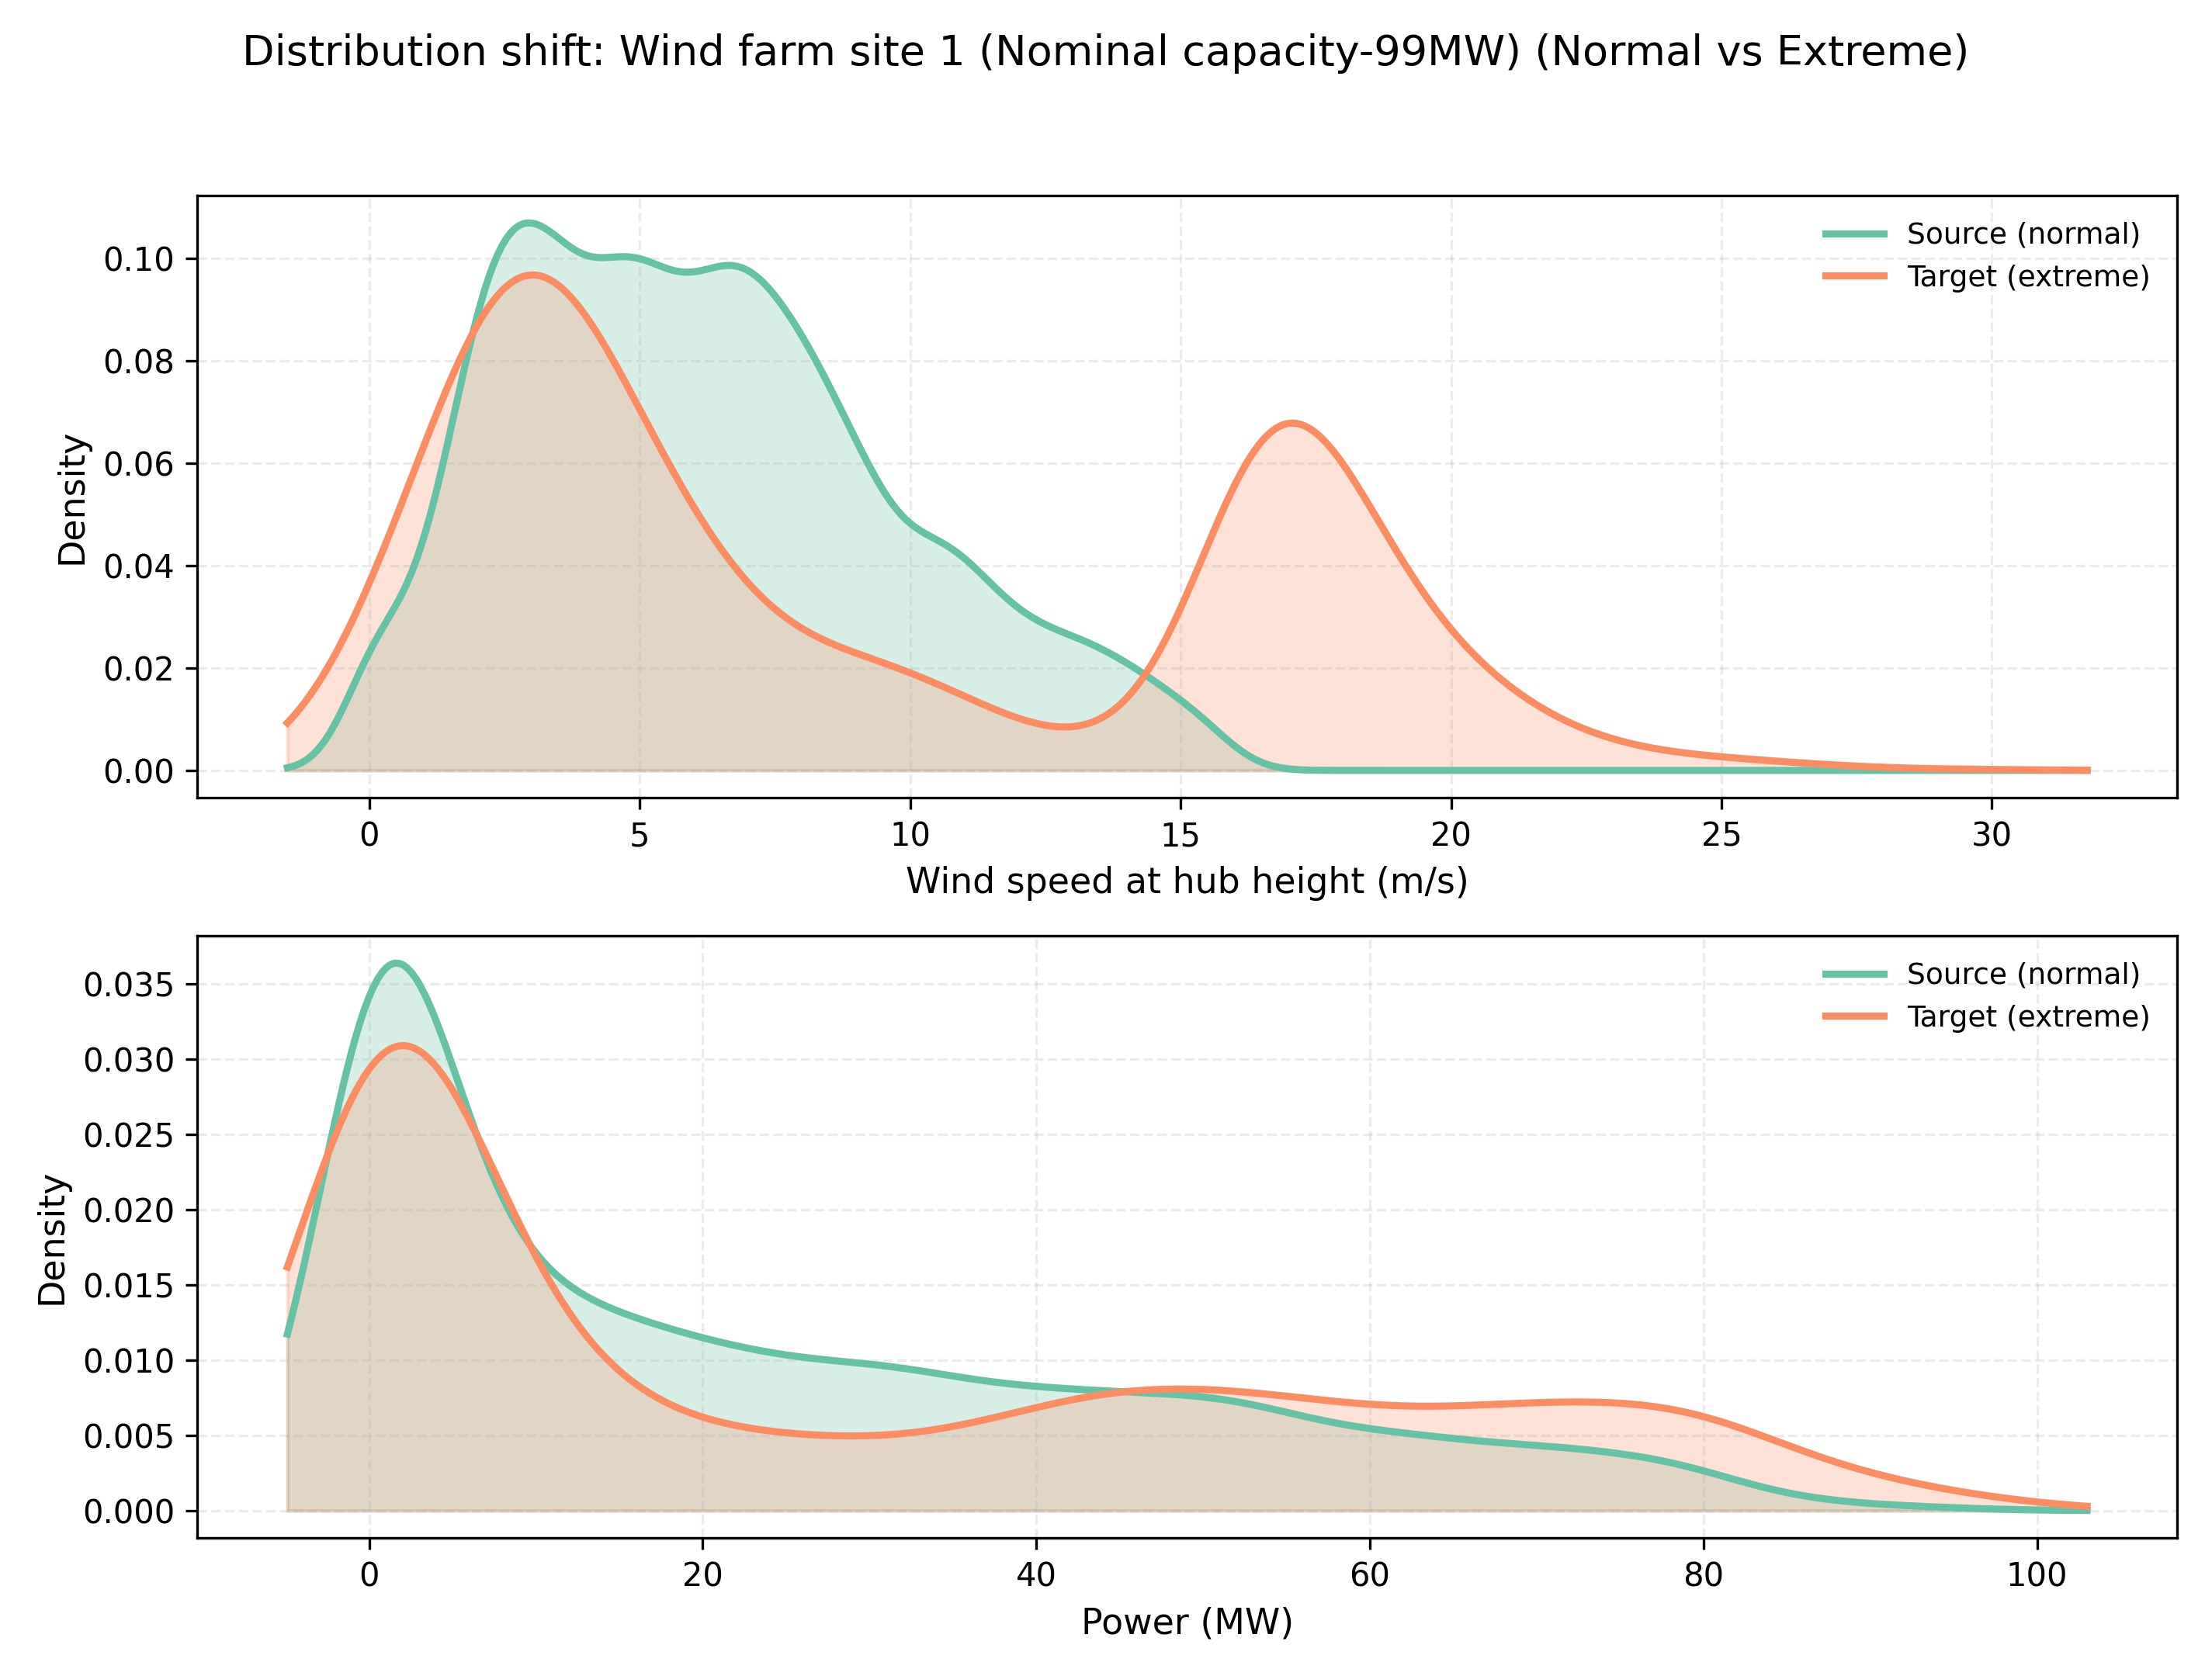
\includegraphics[width=0.48\textwidth]{experiment1/outputs/plots/farm1_domain_shift.jpg}
\hfill
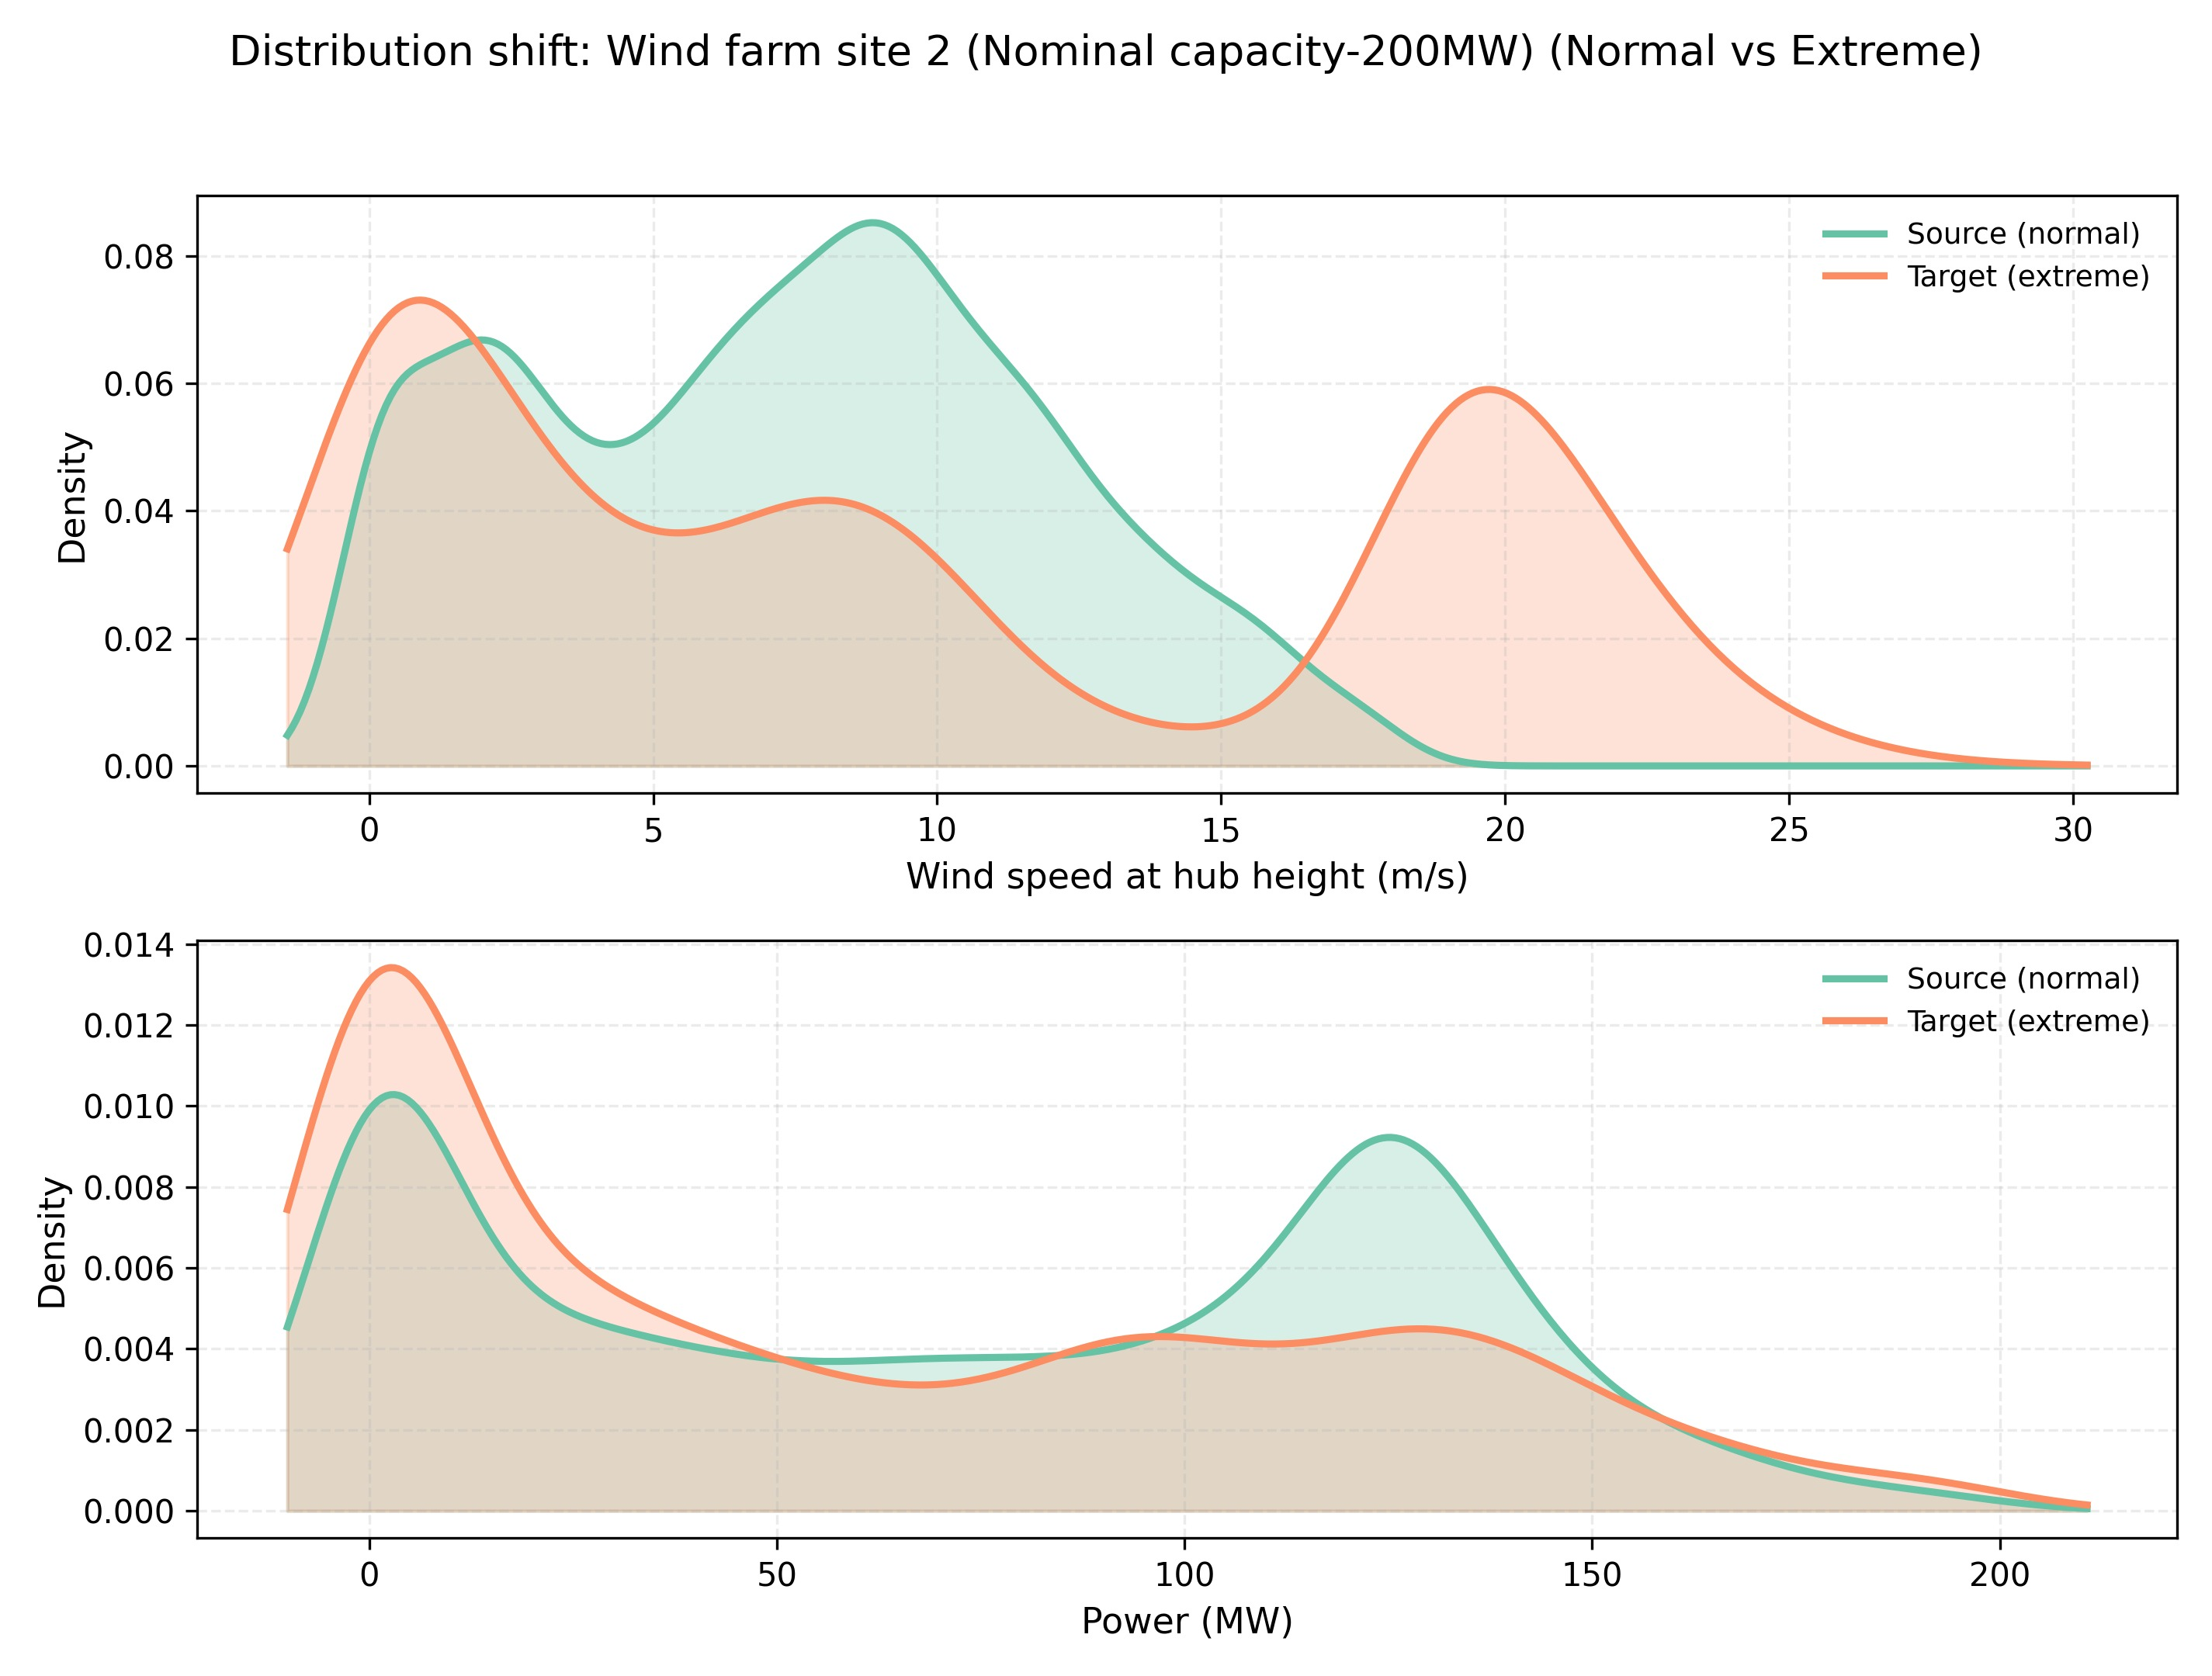
\includegraphics[width=0.48\textwidth]{experiment1/outputs/plots/farm0_domain_shift.jpg}

\vspace{0.3cm}
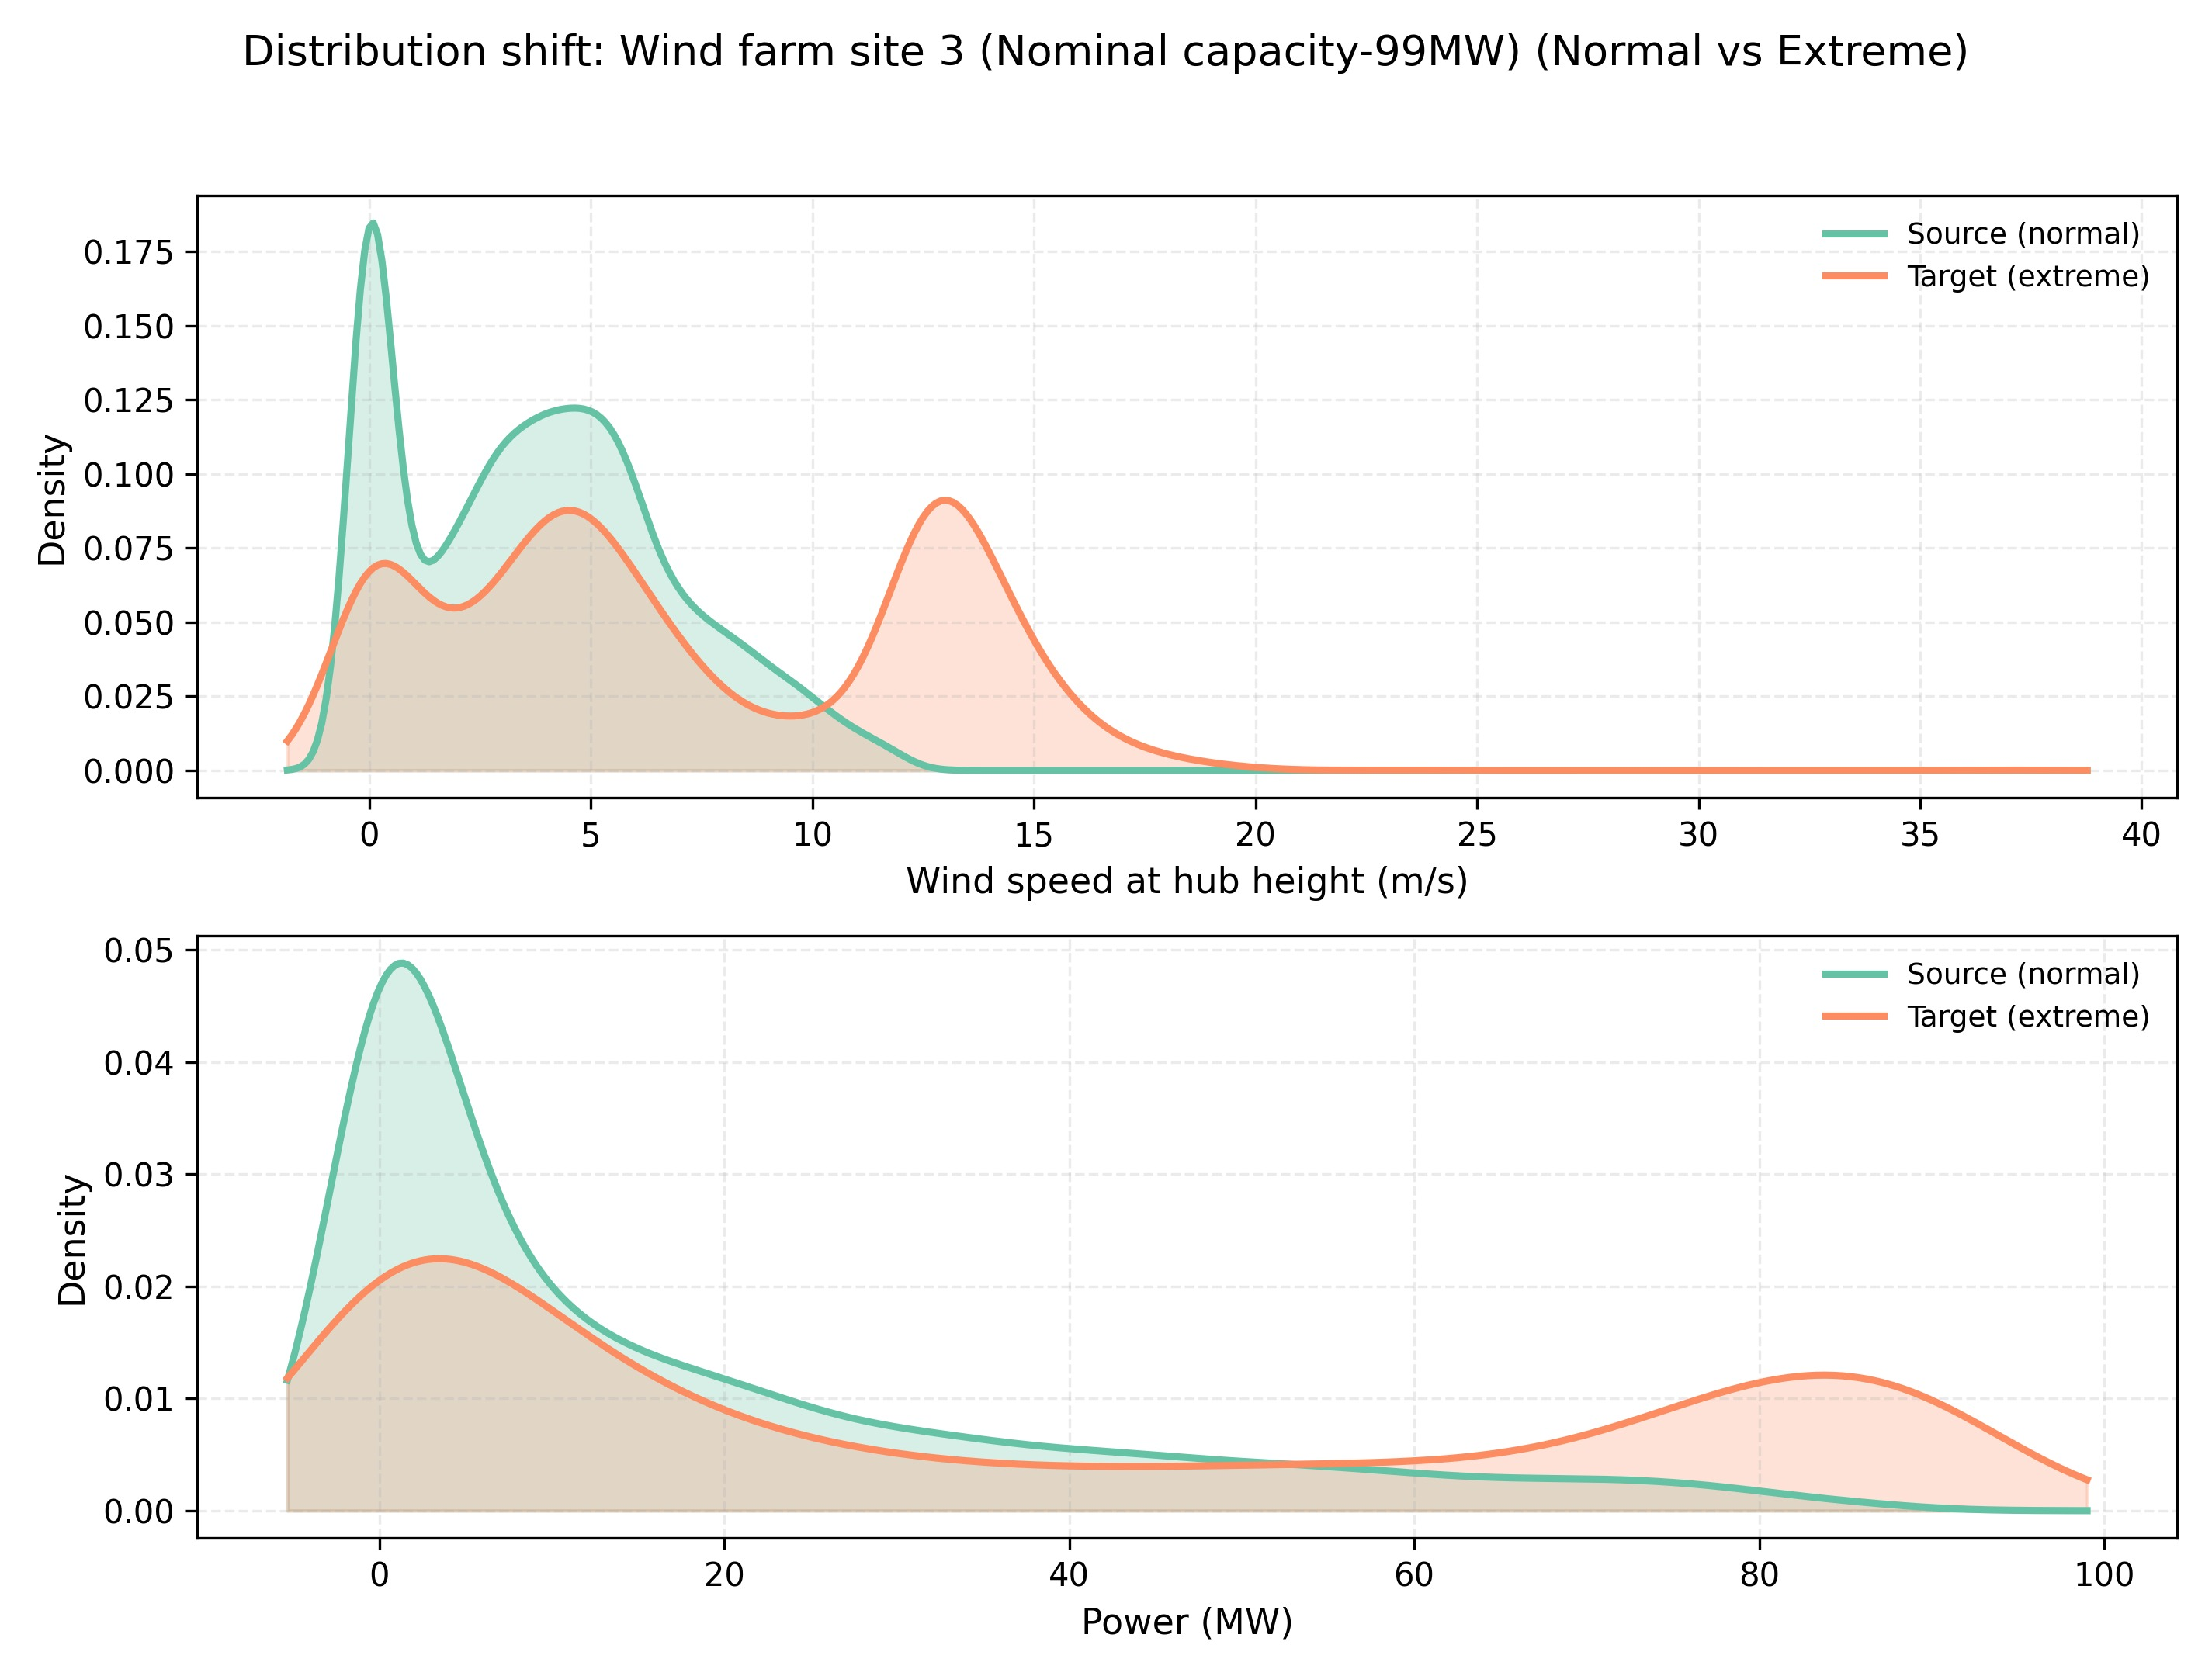
\includegraphics[width=0.48\textwidth]{experiment1/outputs/plots/farm2_domain_shift.jpg}
\hfill
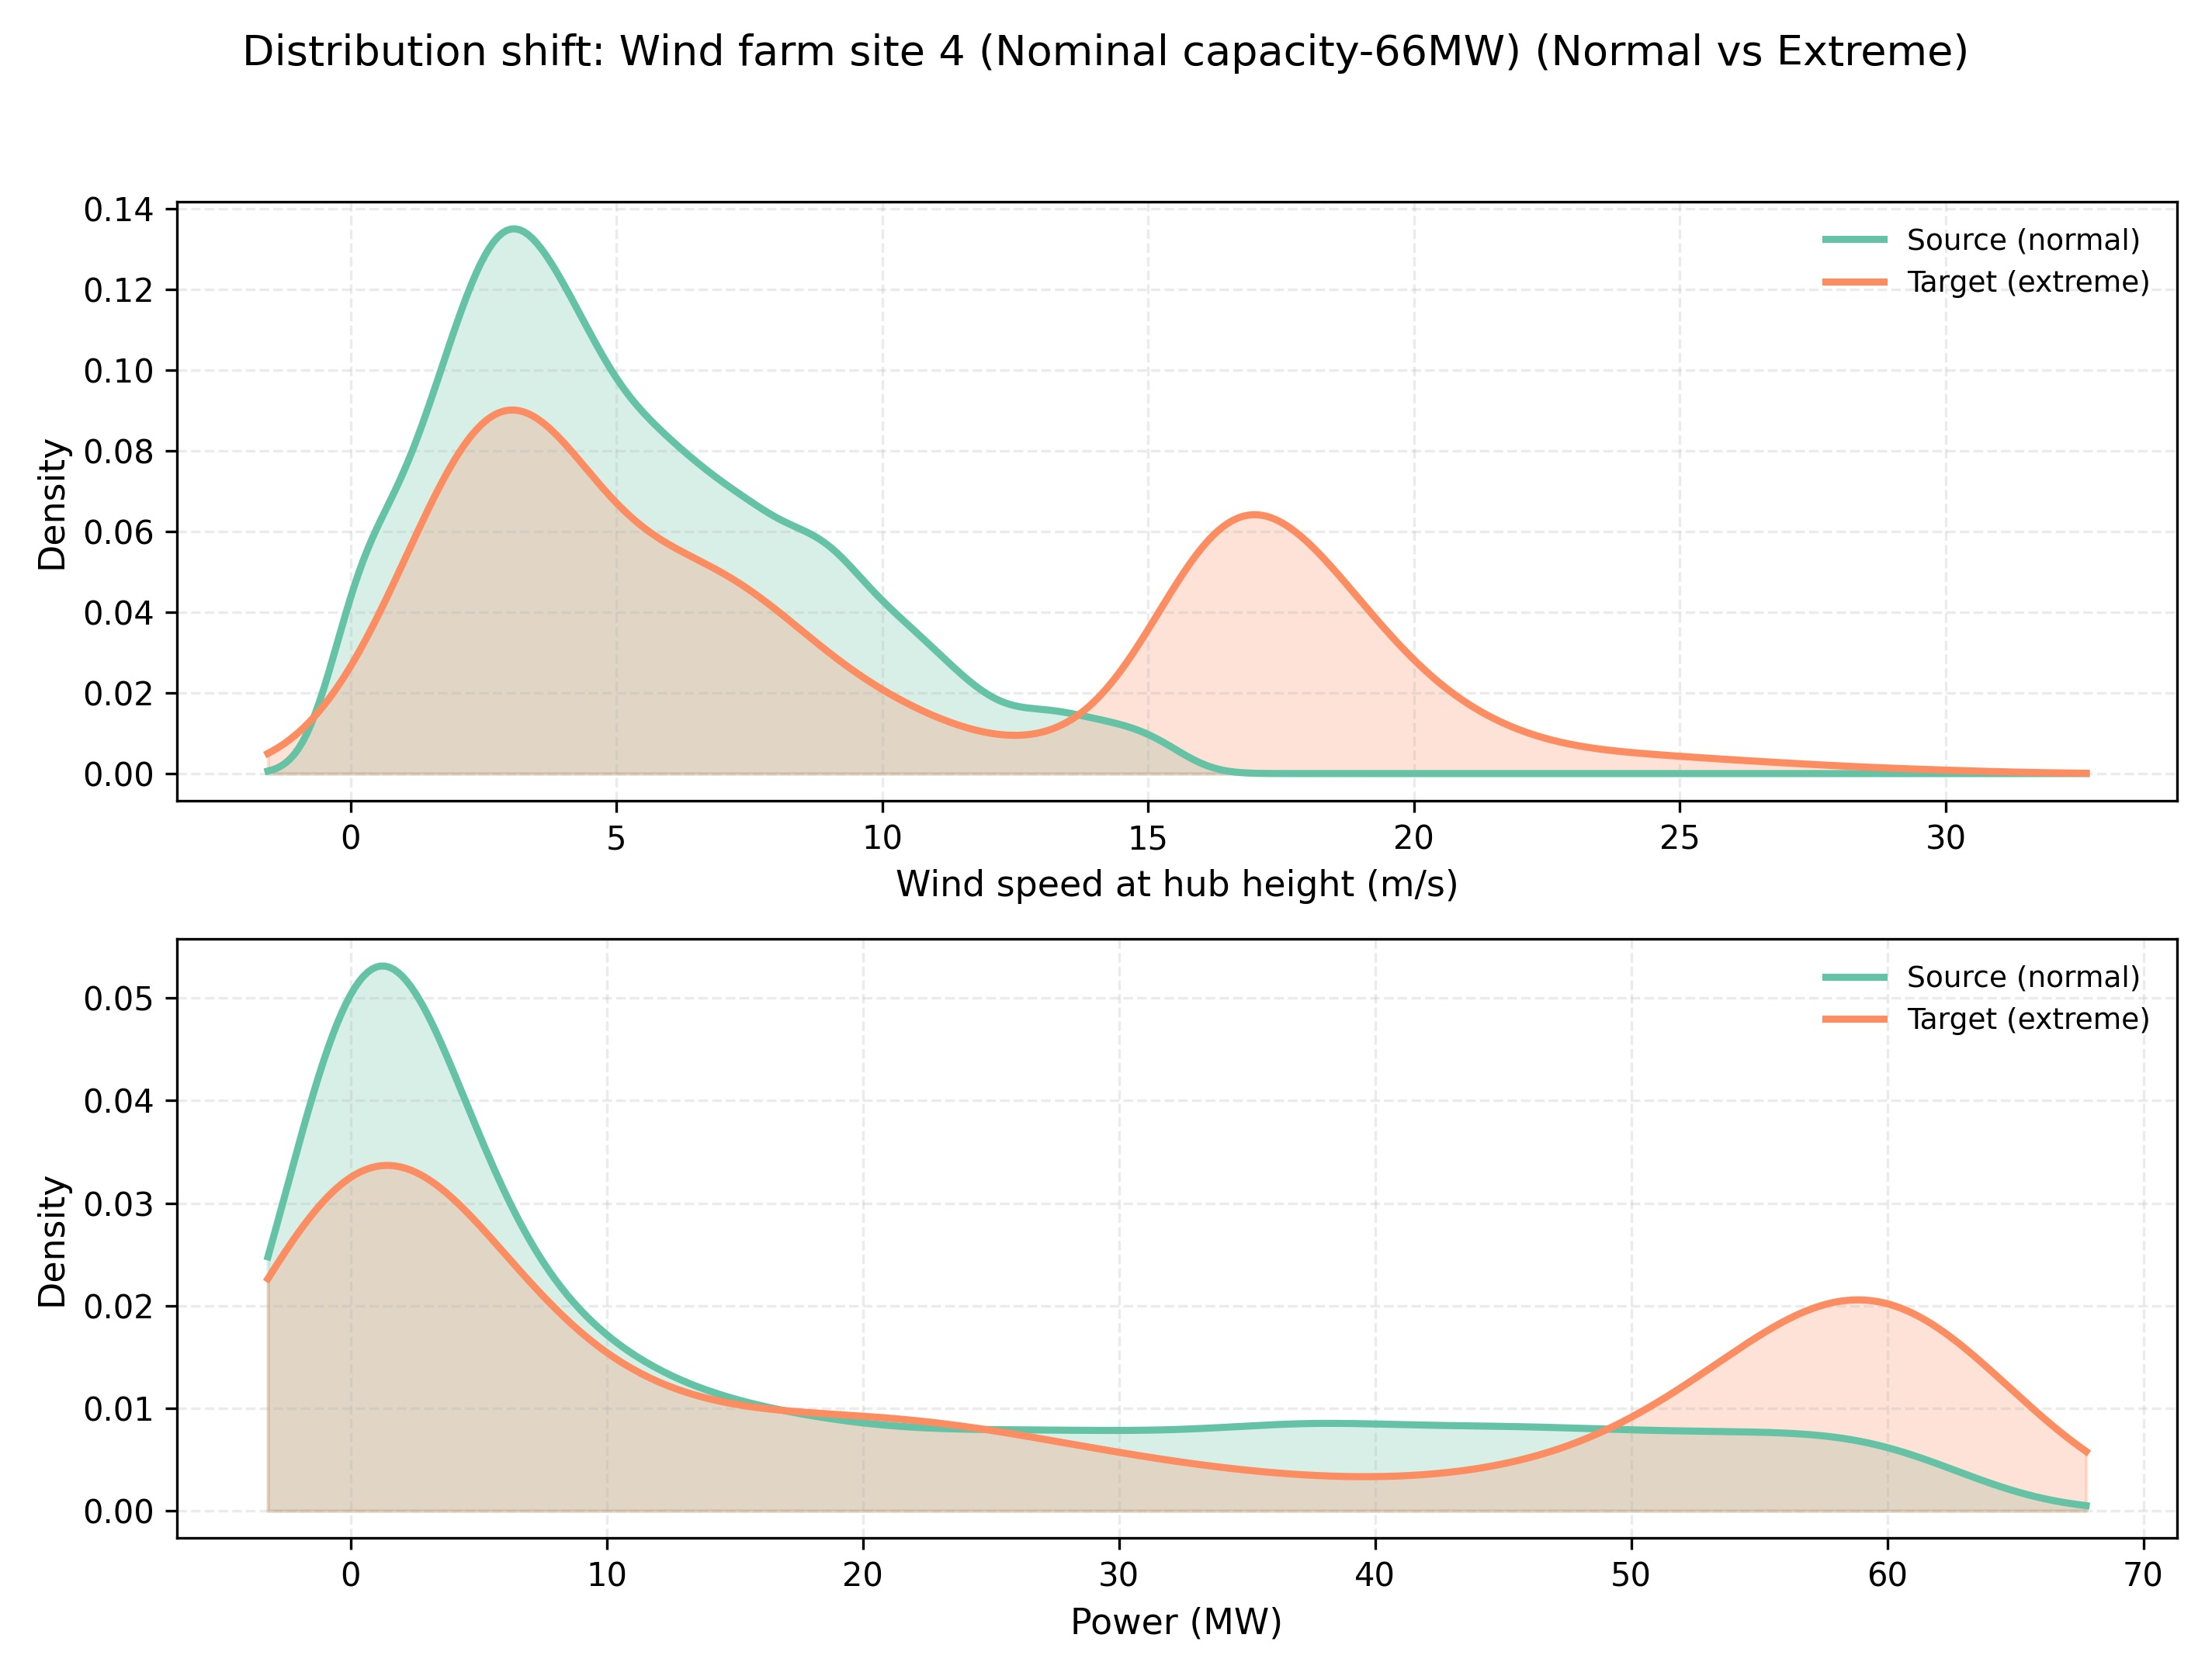
\includegraphics[width=0.48\textwidth]{experiment1/outputs/plots/farm4_domain_shift.jpg}

\vspace{0.3cm}
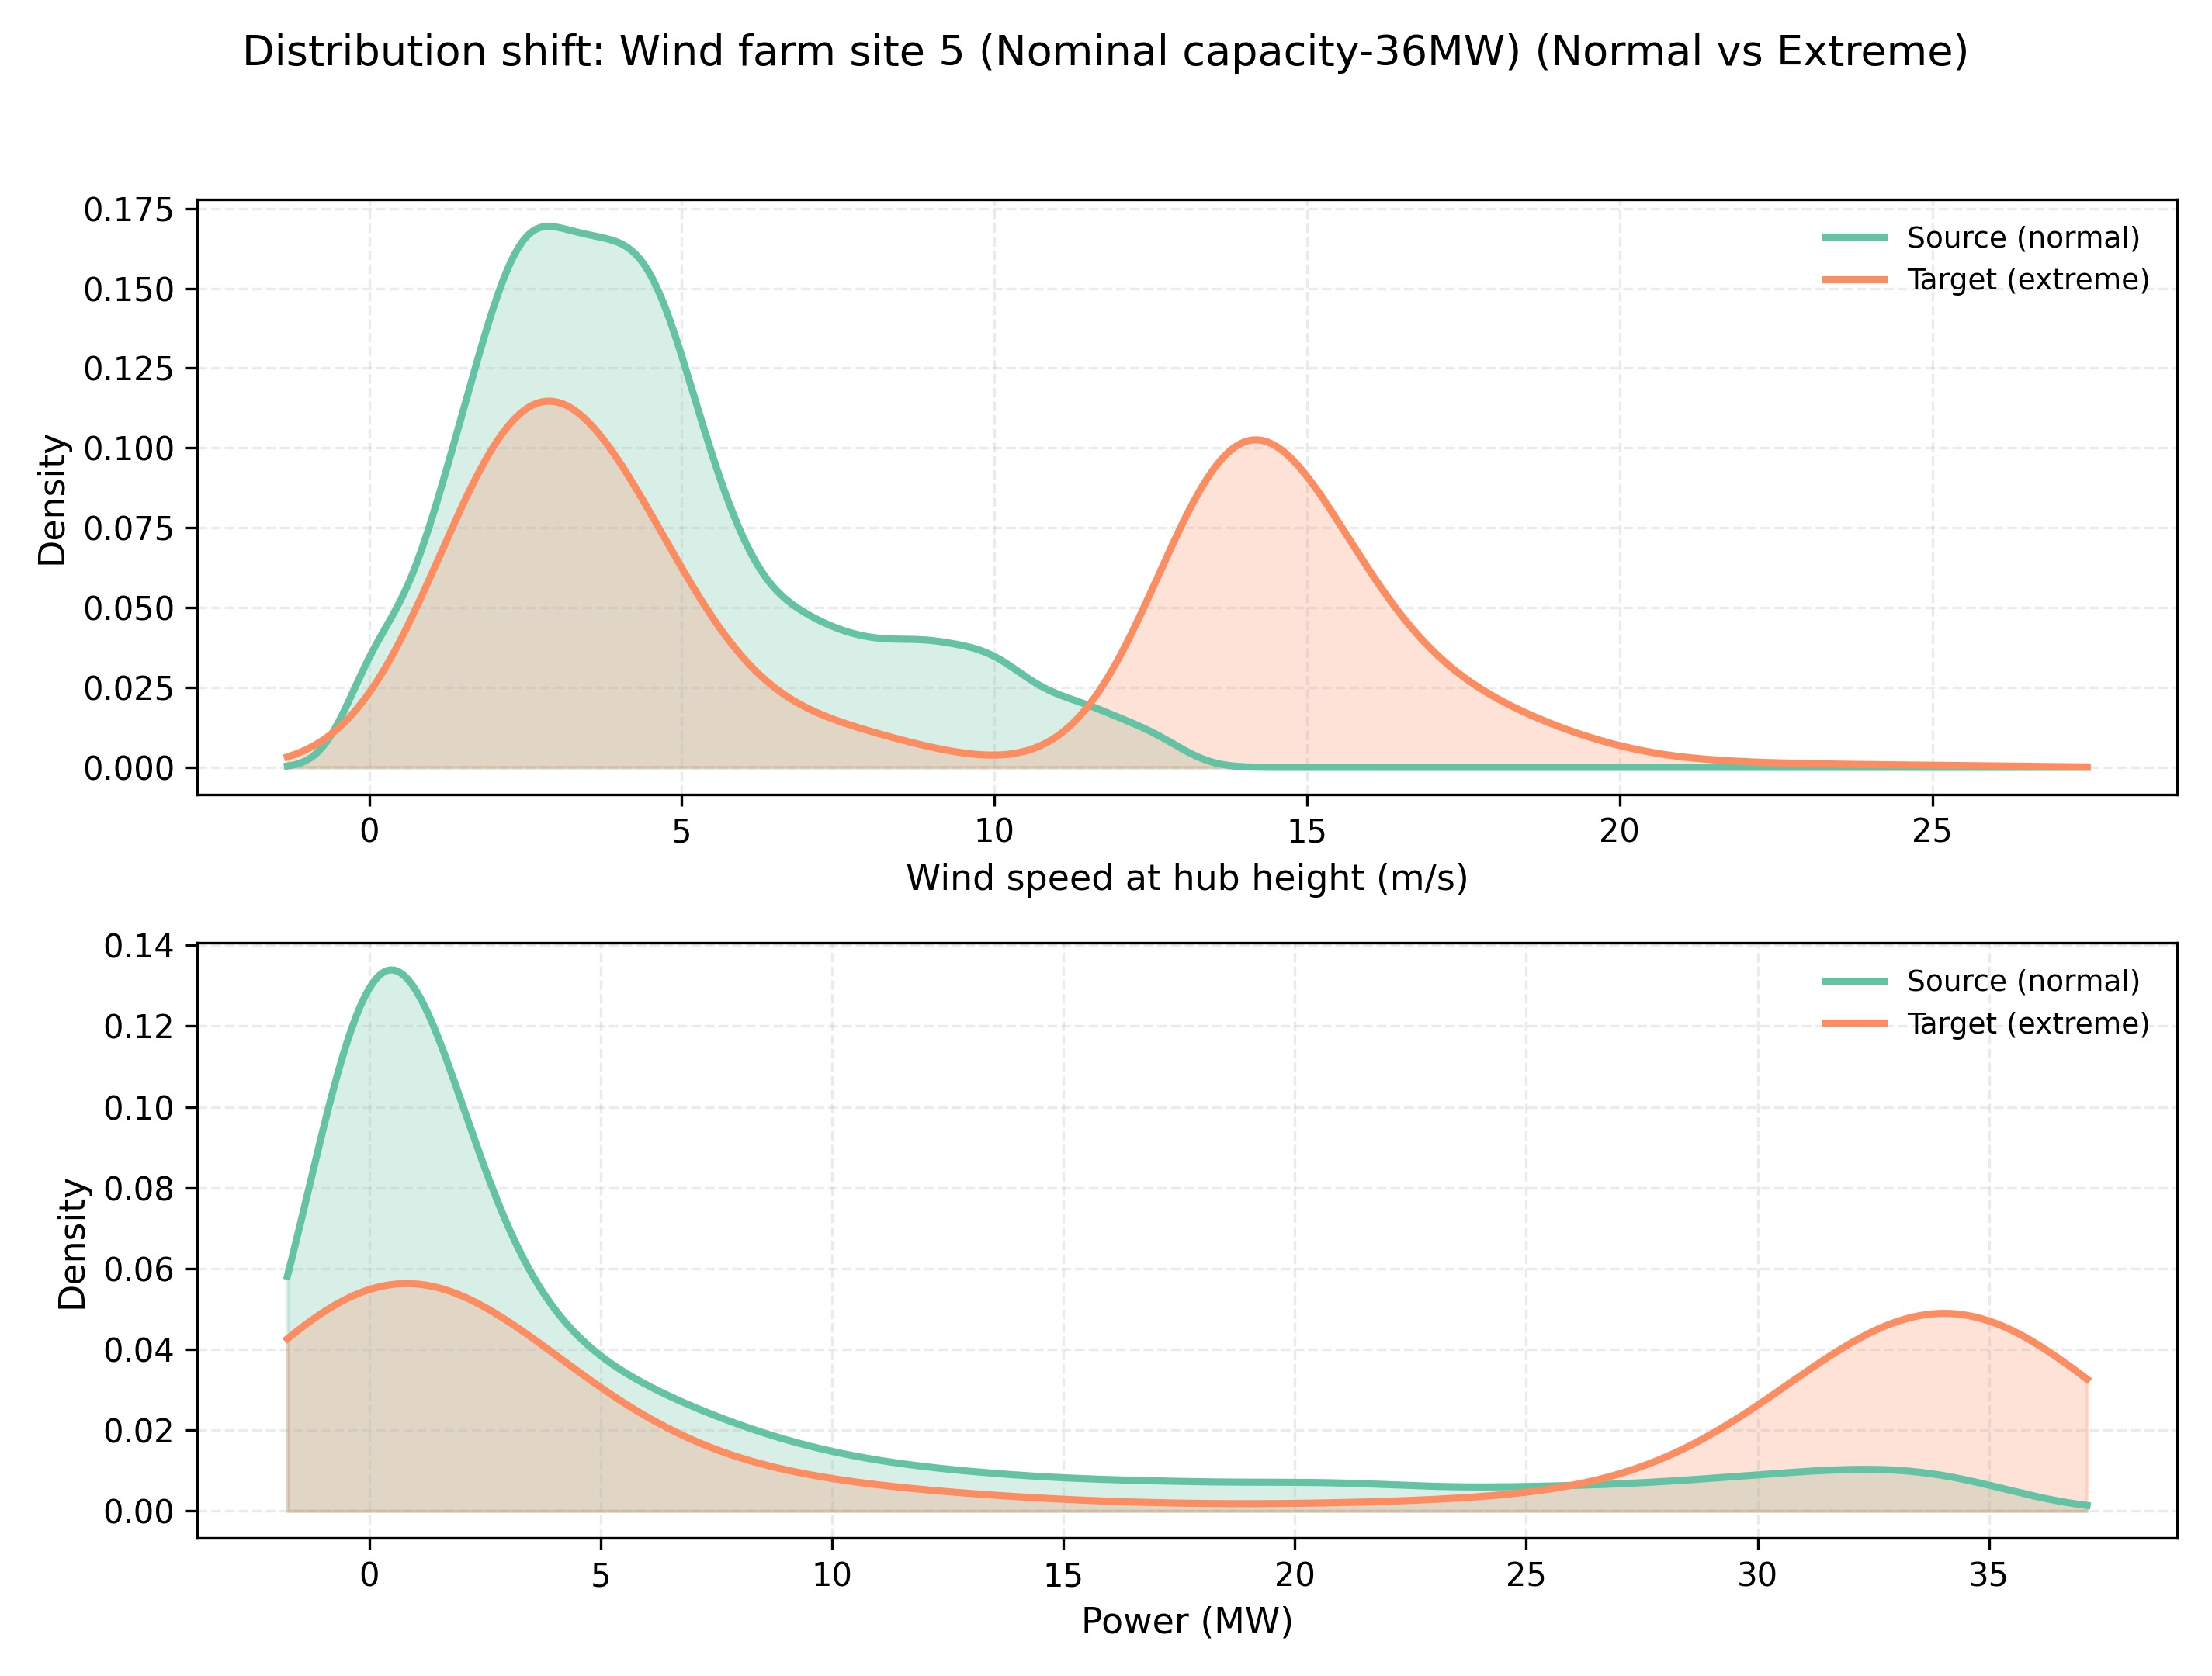
\includegraphics[width=0.48\textwidth]{experiment1/outputs/plots/farm5_domain_shift.jpg}
\hfill
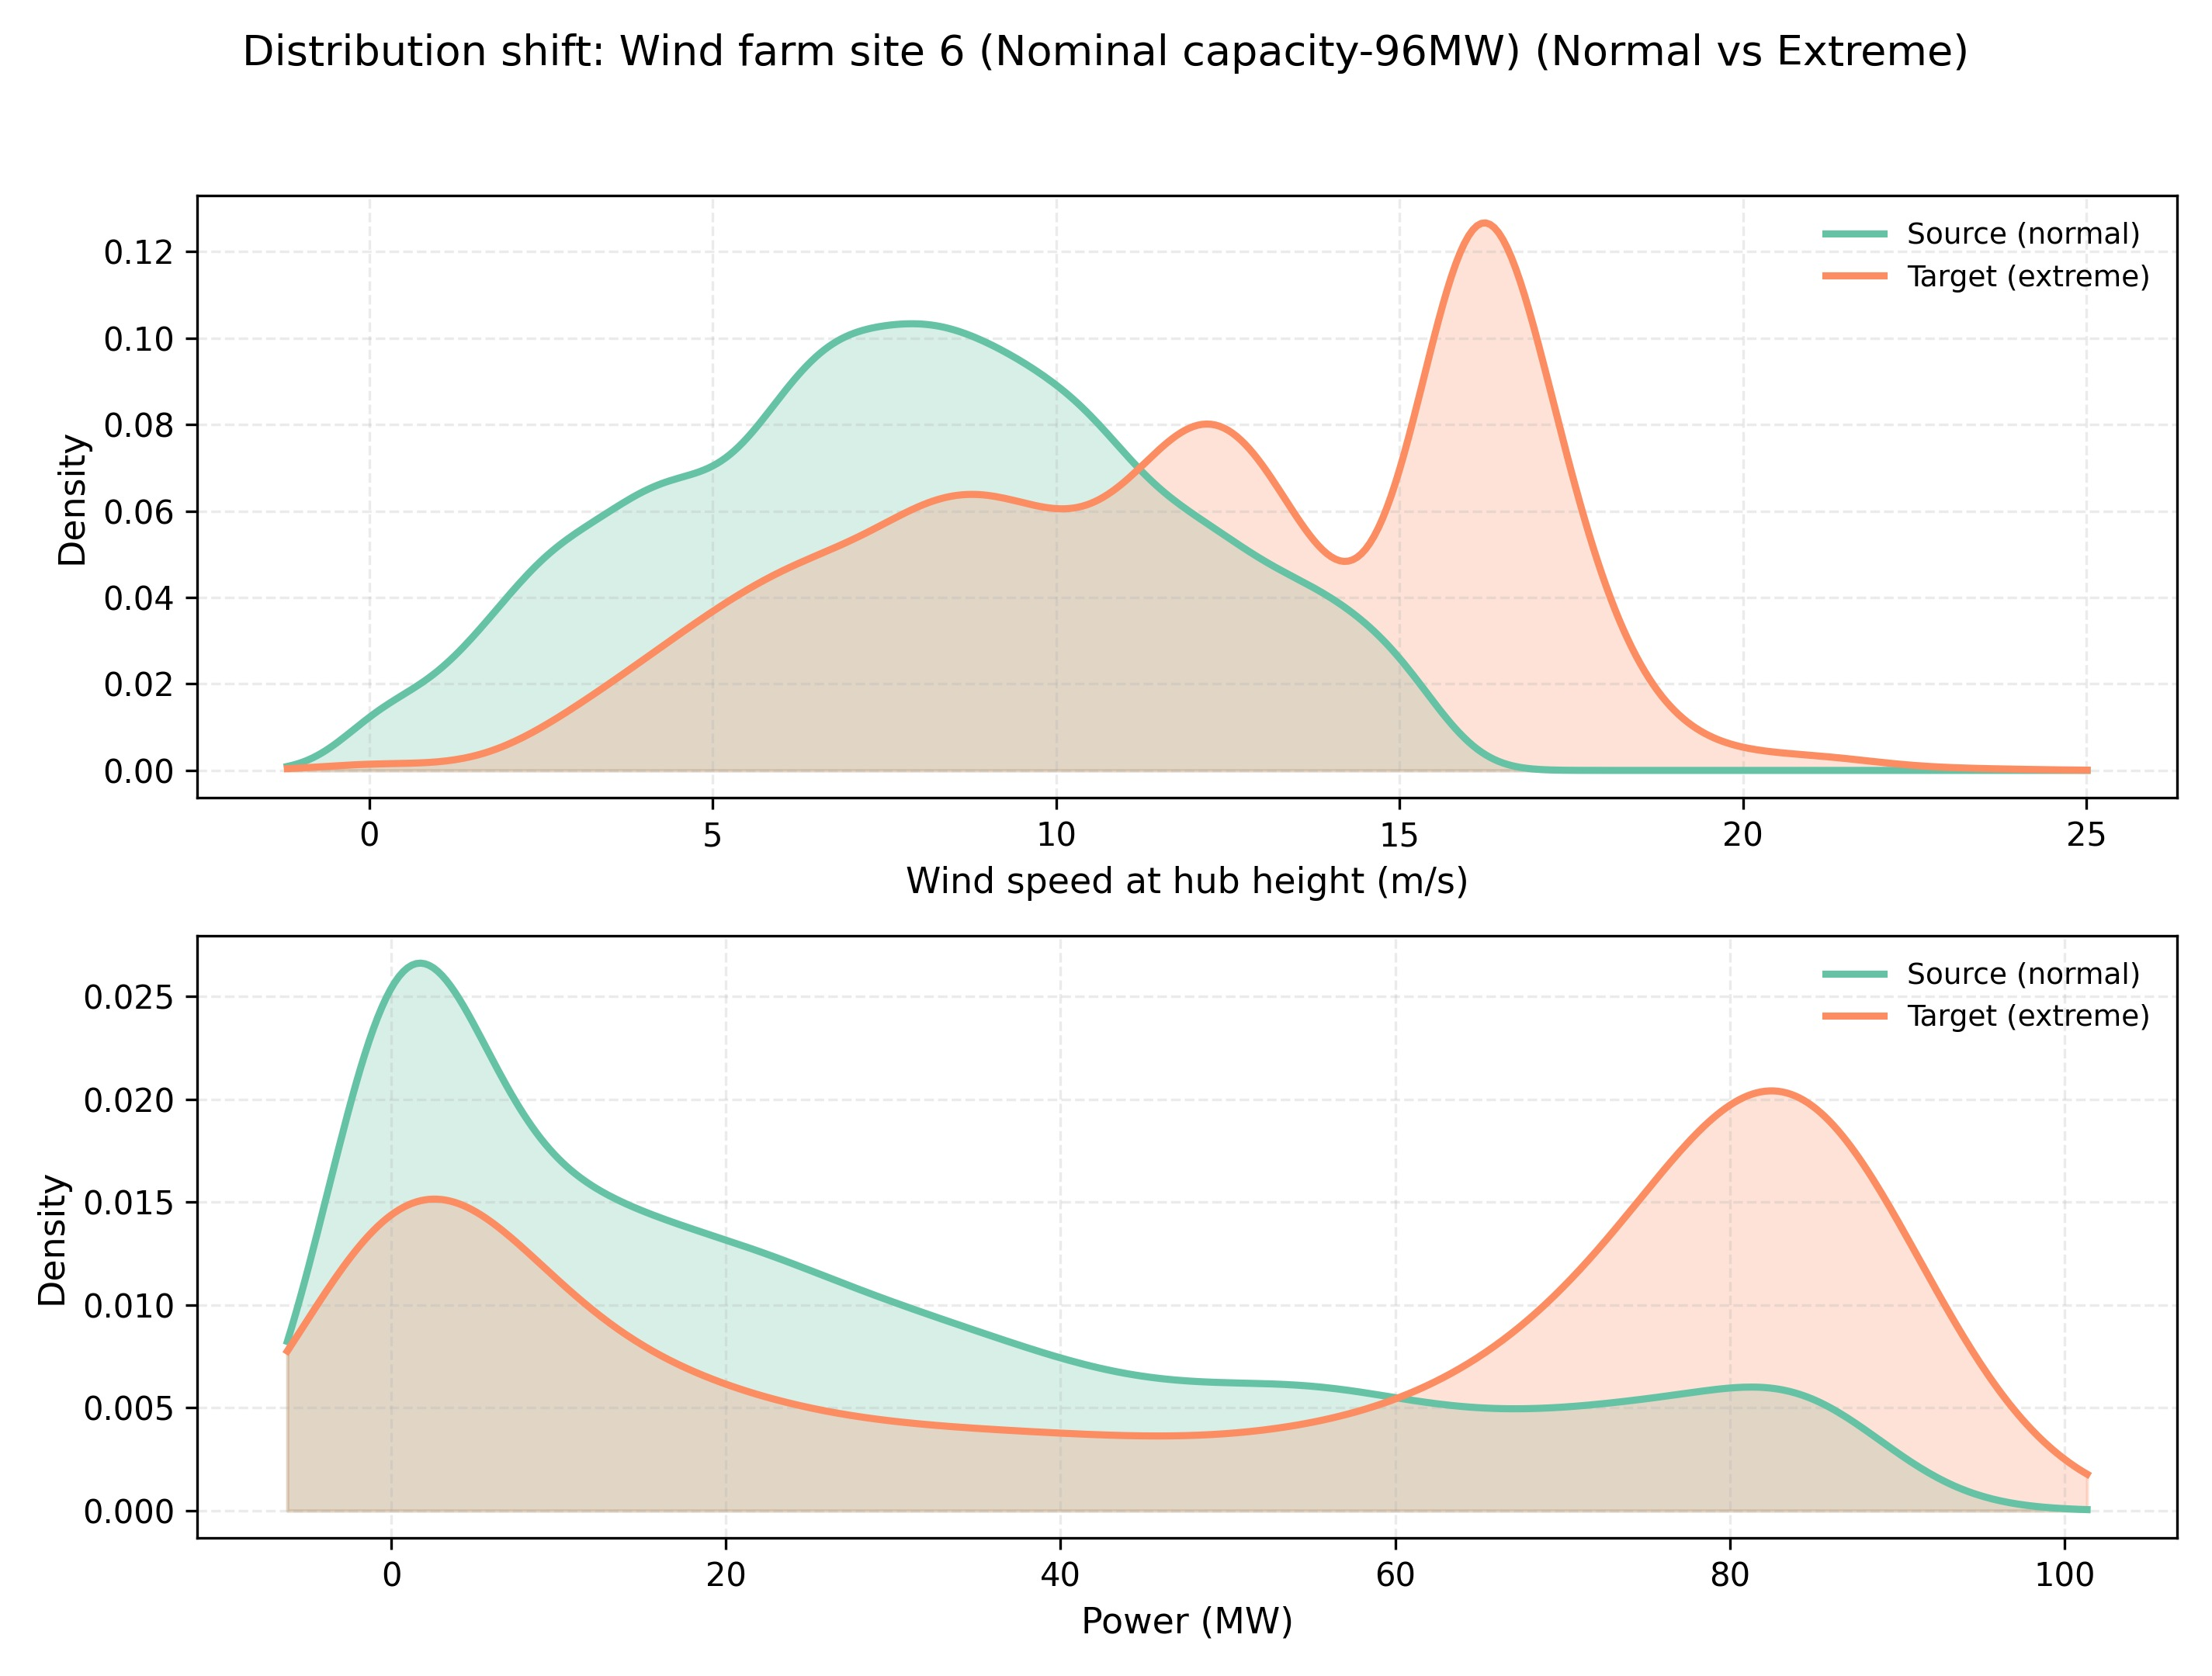
\includegraphics[width=0.48\textwidth]{experiment1/outputs/plots/farm3_domain_shift.jpg}
\refstepcounter{figure}
\par\noindent\textbf{Fig.~\thefigure.} Distribution shift visualization for all six wind farms. From left to right, top to bottom: Site~1 (99\,MW), Site~2 (200\,MW), Site~3 (99\,MW), Site~4 (66\,MW), Site~5 (36\,MW), and Site~6 (96\,MW). Each subplot shows kernel density estimates of wind speed (upper panel) and power output (lower panel) for normal (source) and extreme (target) domains. Site~6 exhibits the most severe domain shift in the power dimension.
\label{fig:domain_shift}
\end{minipage}
\vspace{0.5cm}

\subsubsection{Analysis}

Several observations emerge from Table~\ref{tab:exp1_shift} and Fig.~\ref{fig:domain_shift}. First, all six farms exhibit non-trivial distribution shifts between normal and extreme domains, with KS statistics ranging from 0.116 to 0.460, confirming that extreme weather events induce statistically significant distributional changes in both wind speed and power output. Second, the magnitude of the power distribution shift varies substantially across farms: Farm~6 exhibits a Wasserstein distance of 21.057 in the power dimension, approximately 3.5 times that of Farm~1 (5.964). This disparity reflects differences in turbine control strategies, terrain effects, and the local meteorological characteristics of each site.

Farm~6 (Nominal capacity 96\,MW) ranks first in the composite domain shift metric ($W_1(\text{wind}) + W_1(\text{power}) = 25.117$), indicating the most pronounced distributional discrepancy between its normal and extreme operating regimes. Consequently, \textbf{Farm~6 is selected as the target wind farm for Experiments~2 and~3}, providing the most stringent test bed for evaluating the robustness of transfer learning methods under extreme weather conditions.

%---------------- Experiment 2 --------------------%
\subsection{Experiment 2: Deterministic Point Prediction under Extreme Weather}\label{sec:exp2}

\subsubsection{Objective}

The second experiment evaluates the deterministic point prediction performance of TLQLDMR against a comprehensive set of baseline models on the extreme weather samples of Farm~6. The objective is to demonstrate that the proposed transfer learning mechanism, which leverages abundant normal-weather source domain data to enhance prediction accuracy on scarce extreme-weather target domain data, yields superior forecasting performance compared to models trained solely on the target domain.

\subsubsection{Data Partition}

The data partition for Farm~6 is as follows:
\begin{itemize}
    \item \textbf{Source domain} (normal weather): 66{,}009 samples;
    \item \textbf{Target domain} (extreme weather): 4{,}143 samples, further split into:
    \begin{itemize}
        \item Training set: 3{,}728 samples (90\%);
        \item Test set: 415 samples (10\%).
    \end{itemize}
\end{itemize}

The target domain is split via random shuffling with a fixed seed to ensure reproducibility. All baseline models are trained exclusively on the target domain training set, whereas TLQLDMR additionally incorporates the source domain data through its transfer learning mechanism.

\subsubsection{Baseline Models}

We compare TLQLDMR against six state-of-the-art non-deep-learning models published in 2025, spanning SVM variants, tree-based ensembles, and random forest methods specifically designed for wind power forecasting:

\begin{enumerate}
    \item \textbf{HHO-SVR} \citep{houssein2025hho}: Support Vector Regression with hyperparameters optimized by the Harris Hawks Optimization metaheuristic;
    \item \textbf{FLSVR} \citep{meena2025flsvr}: A functional iterative method for solving the Lagrangian dual of SVR, offering improved convergence properties;
    \item \textbf{ARA-SVR} \citep{duan2025ara}: SVR with Associated Road Analysis for feature selection, originally proposed for short-term traffic flow prediction;
    \item \textbf{KMeans-GBT} \citep{rizkallah2025kmeans}: A two-stage model combining KMeans clustering with Gradient Boosted Trees to capture heterogeneous input--output relationships;
    \item \textbf{RF-WPF} \citep{mustaffa2025rf}: A Random Forest model tailored for wind power forecasting with optimized tree depth and feature subsampling;
    \item \textbf{BRF-WPF} \citep{chen2025brf}: Broad Random Forest integrating Broad Learning System feature expansion with Random Forest regression for short-term wind power prediction.
\end{enumerate}

All baseline models use hyperparameters consistent with their respective publications or default configurations, without extensive grid search, to ensure a fair comparison that reflects each method's out-of-the-box performance.

\subsubsection{TLQLDMR Configuration}

The key hyperparameters of TLQLDMR are determined via a structured search on the validation set (20\% held out from the target training data). The optimal configuration is: $\lambda_1 = 5 \times 10^{-4}$, $\lambda_2 = 1 \times 10^{-4}$, $C_S = 0.05$, $C_T = 150$, $\gamma_{\text{kernel}} = 0.002$, Nystr\"{o}m components $m = 1{,}200$, learning rate $\eta = 0.01$, epochs $= 64$, batch size $= 256$, and $\tau = 0.5$ (median regression for point prediction). The large ratio $C_T / C_S = 3{,}000$ reflects the asymmetric weighting strategy that assigns substantially higher importance to the scarce extreme weather samples.

\subsubsection{Results}

Table~\ref{tab:exp2_results} presents the test set performance of all models on the extreme weather domain of Farm~6.

\begin{table}[ht]
\centering
\caption{Deterministic point prediction results on the extreme weather test set of Farm~6 (96\,MW). Best results are highlighted in bold.}
\setlength{\tabcolsep}{3.5mm}
\begin{tabular}{lccc}
\toprule
Model & RMSE & MAE & $R^2$ \\
\midrule
HHO-SVR    & 7.603 & 5.530 & 0.9537 \\
FLSVR      & 8.794 & 6.301 & 0.9381 \\
ARA-SVR    & 9.246 & 5.954 & 0.9316 \\
KMeans-GBT & 9.620 & 6.695 & 0.9259 \\
RF-WPF     & 7.967 & 5.344 & 0.9492 \\
BRF-WPF    & 9.719 & 6.870 & 0.9244 \\
\textbf{TLQLDMR} & \textbf{7.476} & \textbf{5.348} & \textbf{0.9553} \\
\bottomrule
\end{tabular}
\label{tab:exp2_results}
\end{table}


\subsubsection{Analysis}

TLQLDMR achieves the best performance across all primary metrics, with an RMSE of 7.476 and $R^2$ of 0.9553, confirming the effectiveness of the proposed transfer learning framework for extreme weather power prediction. Several key findings merit discussion:

\textbf{(1) Transfer learning provides a consistent advantage.} TLQLDMR outperforms the best non-transfer baseline (HHO-SVR, $R^2 = 0.9537$) by a margin of 0.0016 in $R^2$ and 0.127 in RMSE. While this margin may appear modest in absolute terms, it is achieved under the most challenging domain shift scenario (Farm~6), where the extreme domain contains only 4{,}143 samples. The improvement demonstrates that incorporating source domain knowledge through MMD-based feature alignment and weighted pinball loss effectively compensates for the scarcity of extreme weather training data.

\textbf{(2) SVM-based models exhibit competitive performance.} Among the baselines, HHO-SVR achieves the second-best RMSE (7.603), benefiting from the metaheuristic optimization of SVR hyperparameters. This suggests that kernel methods with well-tuned parameters remain competitive for small-sample regression tasks, even without explicit transfer learning. However, the performance gap between HHO-SVR and TLQLDMR highlights the additional value of domain adaptation.

\textbf{(3) Tree-based models show limitations under extreme conditions.} KMeans-GBT and BRF-WPF yield the lowest $R^2$ values (0.9259 and 0.9244, respectively), indicating that tree-based ensemble methods, while powerful for general regression tasks, may struggle to extrapolate beyond the training distribution when confronted with extreme weather patterns. The clustering mechanism in KMeans-GBT, designed to capture heterogeneous relationships, does not fully compensate for the distributional shift inherent in extreme events.

\textbf{(4) RF-WPF demonstrates strong baseline performance.} The Random Forest model specifically designed for wind power forecasting achieves the second-best MAE (5.344), nearly matching TLQLDMR (5.348). This result underscores the value of domain-specific model design in wind power applications, though RF-WPF's higher RMSE (7.967) suggests greater sensitivity to large prediction errors in the tails of the distribution.

\textbf{(5) MAPE is unreliable for extreme weather evaluation.} We note that the Mean Absolute Percentage Error (MAPE) values for all models are extremely large (on the order of $10^6$--$10^7$), rendering this metric uninformative. This artifact arises because extreme weather samples frequently include near-zero power output (e.g., during cut-out events), causing the denominator of MAPE to approach zero. Consequently, we rely on RMSE and $R^2$ as the primary comparison metrics.

%---------------- Experiment 3 --------------------%
\subsection{Experiment 3: Probabilistic Interval Prediction under Extreme Weather}\label{sec:exp3}

\subsubsection{Objective}

The third experiment extends the evaluation from deterministic point prediction to probabilistic interval prediction. The objective is to assess whether TLQLDMR can produce well-calibrated 95\% prediction intervals (PIs) that achieve adequate coverage probability while maintaining sharp (narrow) interval widths. This is particularly challenging under extreme weather conditions, where the inherent volatility of wind power amplifies the tension between reliability and sharpness.

\subsubsection{Data Partition}

To support the calibration-based interval prediction framework, the target domain data is partitioned into four subsets:
\begin{itemize}
    \item Training set: 2{,}983 samples (for model fitting);
    \item Validation set: 559 samples (for hyperparameter selection and width scaling);
    \item Calibration set: 745 samples (for Conformalized Quantile Regression adjustment);
    \item Test set: 415 samples (for final evaluation).
\end{itemize}

\subsubsection{Calibration Strategy}

All models employ a two-stage calibration procedure based on Conformalized Quantile Regression (CQR):
\begin{enumerate}
    \item \textbf{Conformal adjustment}: The model first predicts intervals on the calibration set. The conformal quantile $\hat{q}$ is computed as the $(1 - \alpha)$-quantile of the nonconformity scores $\max(L_i - y_i, y_i - U_i)$, ensuring finite-sample coverage guarantees;
    \item \textbf{Width scaling}: A scaling factor is selected on the validation set to optimize the trade-off between coverage and interval width, subject to the constraint that PICP approaches the target level $1 - \alpha + \delta$, where $\delta = 0.02$ is a safety margin.
\end{enumerate}

All predicted intervals are clipped to the physical range $[0, P_{\text{rated}}]$, where $P_{\text{rated}}$ is the nominal capacity of the wind farm.

\subsubsection{Baseline Models}

The interval prediction baselines are organized into two categories:

\textbf{SVM-based quantile regression variants:}
\begin{enumerate}
    \item \textbf{TSVQR} \citep{tsvqr2023}: Twin Support Vector Quantile Regression, which constructs separate hyperplanes for upper and lower quantiles;
    \item \textbf{UQSVM-SSVQR} \citep{wang2024ssvqr}: Sparse Support Vector Quantile Regression with approximate kernel methods for scalability;
    \item \textbf{NFS-SVQR} \citep{ye2025nfs}: Nonlinear Feature Selection combined with SVQR, published in \textit{Neural Networks} (2025);
    \item \textbf{NuSVR-CI}: $\nu$-Support Vector Regression with CQR-calibrated prediction intervals as a classical SVM baseline.
\end{enumerate}

\textbf{Recent wind power interval prediction models:}
\begin{enumerate}
    \item \textbf{NESCQR} \citep{hu2025nescqr}: Neural Ensemble Search with dynamic Conformalized Quantile Regression, published in \textit{Applied Soft Computing} (2025);
    \item \textbf{NCQ-GBR} \citep{hu2025ncqgbr}: Non-crossing Quantile Gradient Boosted Regression, approximating the improved quantile ensemble learning framework published in \textit{Journal of Renewable and Sustainable Energy} (2025);
    \item \textbf{ENS-KDE} \citep{zhang2024kde}: Ensemble model with Kernel Density Estimation of residuals, implementing the KDE-based interval construction paradigm from recent wind power forecasting literature.
\end{enumerate}

\subsubsection{TLQLDMR Interval Configuration}

For interval prediction, TLQLDMR trains two separate quantile models at $\tau_{\text{low}}$ and $\tau_{\text{high}}$ to construct the lower and upper bounds of the prediction interval. The quantile pair $(\tau_{\text{low}}, \tau_{\text{high}})$ is jointly selected with the hyperparameters on the validation set from the candidate set $\{(0.02, 0.98), (0.05, 0.95), (0.1, 0.9), (0.15, 0.85), (0.2, 0.8)\}$, using a coverage-priority criterion that first ensures PICP $\ge 0.95 + \delta$ and then minimizes PINAW.

\subsubsection{Results}

Table~\ref{tab:exp3_results} presents the interval prediction results on the extreme weather test set of Farm~6 at the 95\% confidence level ($\alpha = 0.05$).

\begin{table*}[ht]
\centering
\caption{Interval prediction results on the extreme weather test set of Farm~6 at 95\% confidence level ($\alpha = 0.05$). Models are sorted by CWC in ascending order. Best results per column are highlighted in bold.}
\setlength{\tabcolsep}{4mm}
\begin{tabular}{lccccc}
\toprule
Model & PICP & MPIW & PINAW & CWC & Winkler \\
\midrule
NCQ-GBR       & \textbf{0.954} & 55.669 & 0.628 & \textbf{0.628} & 109.413 \\
UQSVM-SSVQR  & 0.966 & 91.189 & 1.029 & 1.029 & \textbf{94.027} \\
TSVQR         & 0.908 & \textbf{53.599} & \textbf{0.605} & 46.426 & 117.055 \\
NuSVR-CI      & 0.899 & 48.778 & 0.550 & 46.470 & 114.489 \\
TLQLDMR       & 0.928 & 73.549 & 0.830 & 52.682 & 140.393 \\
NESCQR        & 0.870 & 51.538 & 0.582 & 65.368 & 185.663 \\
ENS-KDE       & 0.848 & 56.951 & 0.643 & 89.570 & 137.402 \\
NFS-SVQR      & 0.829 & 82.838 & 0.935 & 157.786 & 111.298 \\
\bottomrule
\end{tabular}
\label{tab:exp3_results}
\end{table*}

\subsubsection{Analysis}

The interval prediction results reveal a fundamental tension between coverage reliability and interval sharpness under extreme weather conditions:

\textbf{(1) Achieving nominal coverage under extreme conditions is inherently challenging.} Only two models---NCQ-GBR (PICP = 0.954) and UQSVM-SSVQR (PICP = 0.966)---achieve the nominal 95\% coverage target. This observation underscores the difficulty of probabilistic forecasting under distribution shift: the extreme weather test set contains patterns that are underrepresented in the training data, making it challenging for models to reliably bound the prediction uncertainty.

\textbf{(2) A pronounced coverage--sharpness trade-off is observed.} The two models that achieve adequate coverage do so at the cost of substantially wider intervals. UQSVM-SSVQR achieves the highest PICP (0.966) but produces the widest intervals (MPIW = 91.189, PINAW = 1.029), meaning the average interval width exceeds the range of observed power values. NCQ-GBR achieves a better balance (PICP = 0.954, PINAW = 0.628), yielding the best CWC score (0.628). This trade-off is a direct consequence of the extreme domain's high volatility.

\textbf{(3) TLQLDMR demonstrates moderate performance.} TLQLDMR achieves a PICP of 0.928, ranking third among all models but falling short of the nominal 95\% target. While its coverage exceeds that of NESCQR (0.870), ENS-KDE (0.848), and NFS-SVQR (0.829), the gap to the target coverage indicates that the current transfer learning mechanism, while effective for point prediction, requires further refinement for interval estimation. The moderate interval width (MPIW = 73.549) suggests that the model maintains reasonable sharpness but at the expense of reliability.

\textbf{(4) Classical SVM baselines exhibit competitive sharpness.} TSVQR and NuSVR-CI produce the narrowest intervals (PINAW = 0.605 and 0.550, respectively) but fail to achieve adequate coverage (PICP = 0.908 and 0.899). This pattern is consistent with the known behavior of SVM-based quantile regression: the maximum margin principle tends to produce tight decision boundaries that may not fully capture the tail uncertainty of extreme events.

\textbf{(5) Neural ensemble methods underperform in low-data regimes.} NESCQR, despite its sophisticated neural ensemble architecture with dynamic CQR, achieves only 0.870 coverage with a Winkler score of 185.663---the worst among all models. This suggests that the neural ensemble's flexibility may lead to overfitting on the small extreme weather training set, producing poorly calibrated intervals. The result highlights the advantage of kernel-based methods with explicit regularization in data-scarce scenarios.

%---------------- Discussion --------------------%
\subsection{Discussion}\label{sec:discussion}

The experimental results yield the following key findings:

\textbf{Transfer learning improves point prediction under extreme conditions.} Experiment~2 demonstrates that TLQLDMR's dual-space adaptation mechanism---combining MMD-based feature alignment with weighted pinball loss---successfully transfers knowledge from the abundant normal-weather domain to the scarce extreme-weather domain, achieving the best deterministic prediction performance ($R^2 = 0.9553$, RMSE = 7.476).

\textbf{Interval prediction under distribution shift remains challenging.} Experiment~3 reveals that achieving both adequate coverage ($\text{PICP} \ge 0.95$) and sharp intervals ($\text{CWC} < 0.5$) simultaneously on the extreme weather test set is difficult for all evaluated methods. TLQLDMR achieves moderate performance (PICP = 0.928) but does not reach the nominal coverage target, suggesting that the current formulation requires further development in uncertainty quantification under distribution shift. Potential directions include adaptive conformal prediction with covariate shift correction \citep{tibshirani2019conformal}, or distributionally robust optimization approaches.

\textbf{Evaluation metric selection affects model ranking.} The divergent rankings produced by different metrics (e.g., NCQ-GBR ranks first by CWC while UQSVM-SSVQR ranks first by Winkler score) highlight the importance of selecting evaluation criteria aligned with operational requirements. For grid operators prioritizing reliability, PICP should be the primary criterion; for those prioritizing economic efficiency, PINAW or Winkler score may be more appropriate.

\textbf{Limitations.} Several limitations should be acknowledged: (1) the evaluation is conducted on a single wind farm (Farm~6), and generalization to other sites requires further validation; (2) the data partition relies on a single random split without cross-validation, which may introduce partition-dependent variability; (3) the baseline implementations approximate the core ideas of their respective publications, and full-fidelity reproductions may yield different results; (4) the current experiments exclude deep learning models (e.g., Transformer-based architectures), which will be addressed in future work; and (5) TLQLDMR's interval prediction performance, while competitive, does not achieve the nominal 95\% coverage, indicating room for improvement in the uncertainty quantification component.




\section{Conclusion}\label{conclusion}
This paper presents TL-QLDMR for wind power forecasting under extreme events, where target-domain samples are limited and distribution shift is pronounced. The method combines asymmetric variance regularization, MMD-based feature alignment, and weighted pinball loss within a unified transfer-learning quantile framework, with theoretical guarantees on positive definiteness and convergence.

Experimental results show that TL-QLDMR delivers consistent gains in both deterministic and interval forecasting on the most challenging target farm. For point prediction, it achieves the best RMSE (7.478) and $R^2$ (0.9557). For 95\% interval prediction, it attains PICP $=0.959$ together with the best CWC (0.268), indicating a favorable reliability-sharpness trade-off. Under injected noise, TL-QLDMR remains the strongest model across reported point and interval metrics. In addition, the Nystr\"{o}m-SGD solver provides practical scalability, completing the full uncapped training set ($N=69{,}737$) in 5.021 seconds, whereas CVXOPT, Torch-GD, and batch SGD do not remain computationally viable at the same scale.

Future work will focus on extending the framework to multi-site spatiotemporal coupling, adaptive online recalibration under non-stationary weather, and hybrid kernel-deep transfer formulations.

%------------------------ Credit ------------------------
\printcredits


%------------------------ Declaration ------------------------
\section*{Declaration of Competing Interest}
The authors declare that they have no known competing financial interests or personal relationships that could have appeared to influence the work reported in this paper.


%------------------------ Acknowledgments ------------------------
\section*{Acknowledgments}
This work was supported in part by the National Natural Science Foundation of China under Grant 72471109 and Grant 62106205.



%------------------------ Reference ------------------------

%\bibliographystyle{unsrtnat}
% \bibliography{ref}
%\begin{refcontext}[sorting = none]
% \hypersetup{
%   %colorlinks=true,
%   linkcolor=blue,
%   urlcolor=blue
% }

% \bibliographystyle{unsrtnat}
\bibliographystyle{model5-names} 
\bibliography{ref.bib}
%\end{refcontext}

\end{document}
